\chapter{Cube-fx: Mapping to Matrix Multiplications}
\label{sec_4}

In this chapter, we discuss the second optimization approach with the example of Cube-fx. Sec 4.1 introduces the existing algorithms to evaluate special functions as the background. Sec 4.2 discusses the algorithm Cube-fx in detail, which includes two main stages: the computation stage in Sec. 4.2.1 and the preparation stage in Sec. 4.2.2. Sec. 4.3 introduces an enhanced mapping, which aims to enhance Cube-fx for more general cases. Sec. 4.4 evaluates Cube-fx and Sec. 4.5 gives the conclusions.

\section{Background \& Motivation}

\subsection{Taylor Expansion \label{sec:2.3}}

Taylor expansion is a powerful mathematical tool for evaluating a function. It expands infinitely differentiable functions as a series named Taylor series that only contains additions and multiplication. Eq. \ref{eq:taylor} shows the definition of Taylor series, where $f(x)$ is expanded to $n$ degrees at point $a$. The polynomial part of Taylor series is called Taylor polynomial. In the interval of convergence, Taylor polynomial approximates the functions with ignorable errors.

\begin{equation}
    \label{eq:taylor}
    \begin{aligned}
    f(x) = \sum_{k = 0}^{n}\frac{f^{(k)}(a)}{k!}(x - a)^k + o[(x - a) ^ n]
    \end{aligned}
    \end{equation}

One of the common approaches to evaluate a Taylor polynomial is Horner's Method. Evaluating an $n$-degree polynomial in its original form, such as $p(x)$ in Eq. \ref{eq:horner}, requires $(n^2 + n)/2$ multiplications and $n$ additions. Horner's Method reduces this to $n$ multiplications and additions by transforming the polynomial into a combination of $n$ linear polynomials. Estrin's Scheme \cite{DBLP:conf/aieeire/Estrin60} further decomposes the polynomial into independent sub-polynomials that can be computed in parallel, requiring $(n - 1)$ multiplications and additions, along with an additional $\log_2{n}$ squarings, when $n$ is a power of 2. Motzkin's Method \cite{motzkin1955evaluation}, using coefficient pre-processing, divides the polynomial into several sub-polynomials. For a 4th-degree polynomial, Motzkin's Method requires only 2 multiplications and 5 additions, compared to 4 multiplications and additions with Horner's Method, making it more efficient on hardware where multiplications are costly. These methods, as injective functions, can naturally be adapted for parallel implementation using SIMD on vectorized units when dealing with large inputs. However, as discussed in Sec. \ref{Sec:1_1_2}, current AI processors perform poorly on vectorized operations, leading to performance losses. Therefore, instead of reducing the number of vectorized operations, leveraging Matrix MACs for computation will be more effective on AI processors.

\begin{equation}
    \label{eq:horner}
    \begin{aligned}
    f_a(x) &= a_n x^n + a_{n - 1}x^{n - 1} + ... + a_1 x + a_0 \\
         &= (((a_n x + a_{n - 1}) x + a_{n - 2})x + ... + a_1) x + a_0 
    \end{aligned}
    \end{equation}

Furthermore, in applications such as optimization problems \cite{boyd2004convex}, feature extraction \cite{deller1993discrete}, or combinations of multiple activations \cite{DBLP:conf/icpr/ManessiR18}, data often need to be processed by multiple functions. Methods like Horner's Method, Estrin's Scheme, and Motzkin's Method handle each function independently, requiring redundant calculations. For example, consider two functions, $f_a(x)$ in Eq. \ref{eq:horner} and $f_b(x)$, which share the same input $x$. Taking Horner's Method as an example, the intermediate result from computing $f_a(x)$, such as $(a_nx + a_{n-1})$, is discarded immediately after computing $f_a(x)$ and cannot be reused for $f_b(x)$. This results in repeating the evaluation process for each function. In contrast, using the original form of Taylor polynomials allows for common intermediate results, such as the sequence of powers $(x^n, x^{n-1}, \ldots, x)$, to be reused by multiple functions. If $f_a(x)$ generates this sequence, $f_b(x)$ and other functions can reuse it for their computations and reduce redundancy. However, generating this sequence is time-consuming with the vectorized units on AI processors, potentially offsetting the benefits of intermediate result reuse because of the inefficiencies in vectorized operations.

\section{Cube-fx Algorithm \label{sec:3}}

Fig. \ref{fig:overview} gives an overview of Cube-fx. It contains two main stages: the preparation stage to generate the intermediate sequence $(x, x^2, x^3, ...)$ from input $x$ and the computation stage to evaluate multiple functions in parallel. Compared with previous implementations composed of vectorized operations, either stage of Cube-fx contains one matrix multiplication as the key mapping step accelerated by the Matrix MACs. Each matrix of the matrix multiplications is specially designed and fixed, which aims to avoid extra matrix generation. 

\begin{figure}[t]
    \centering{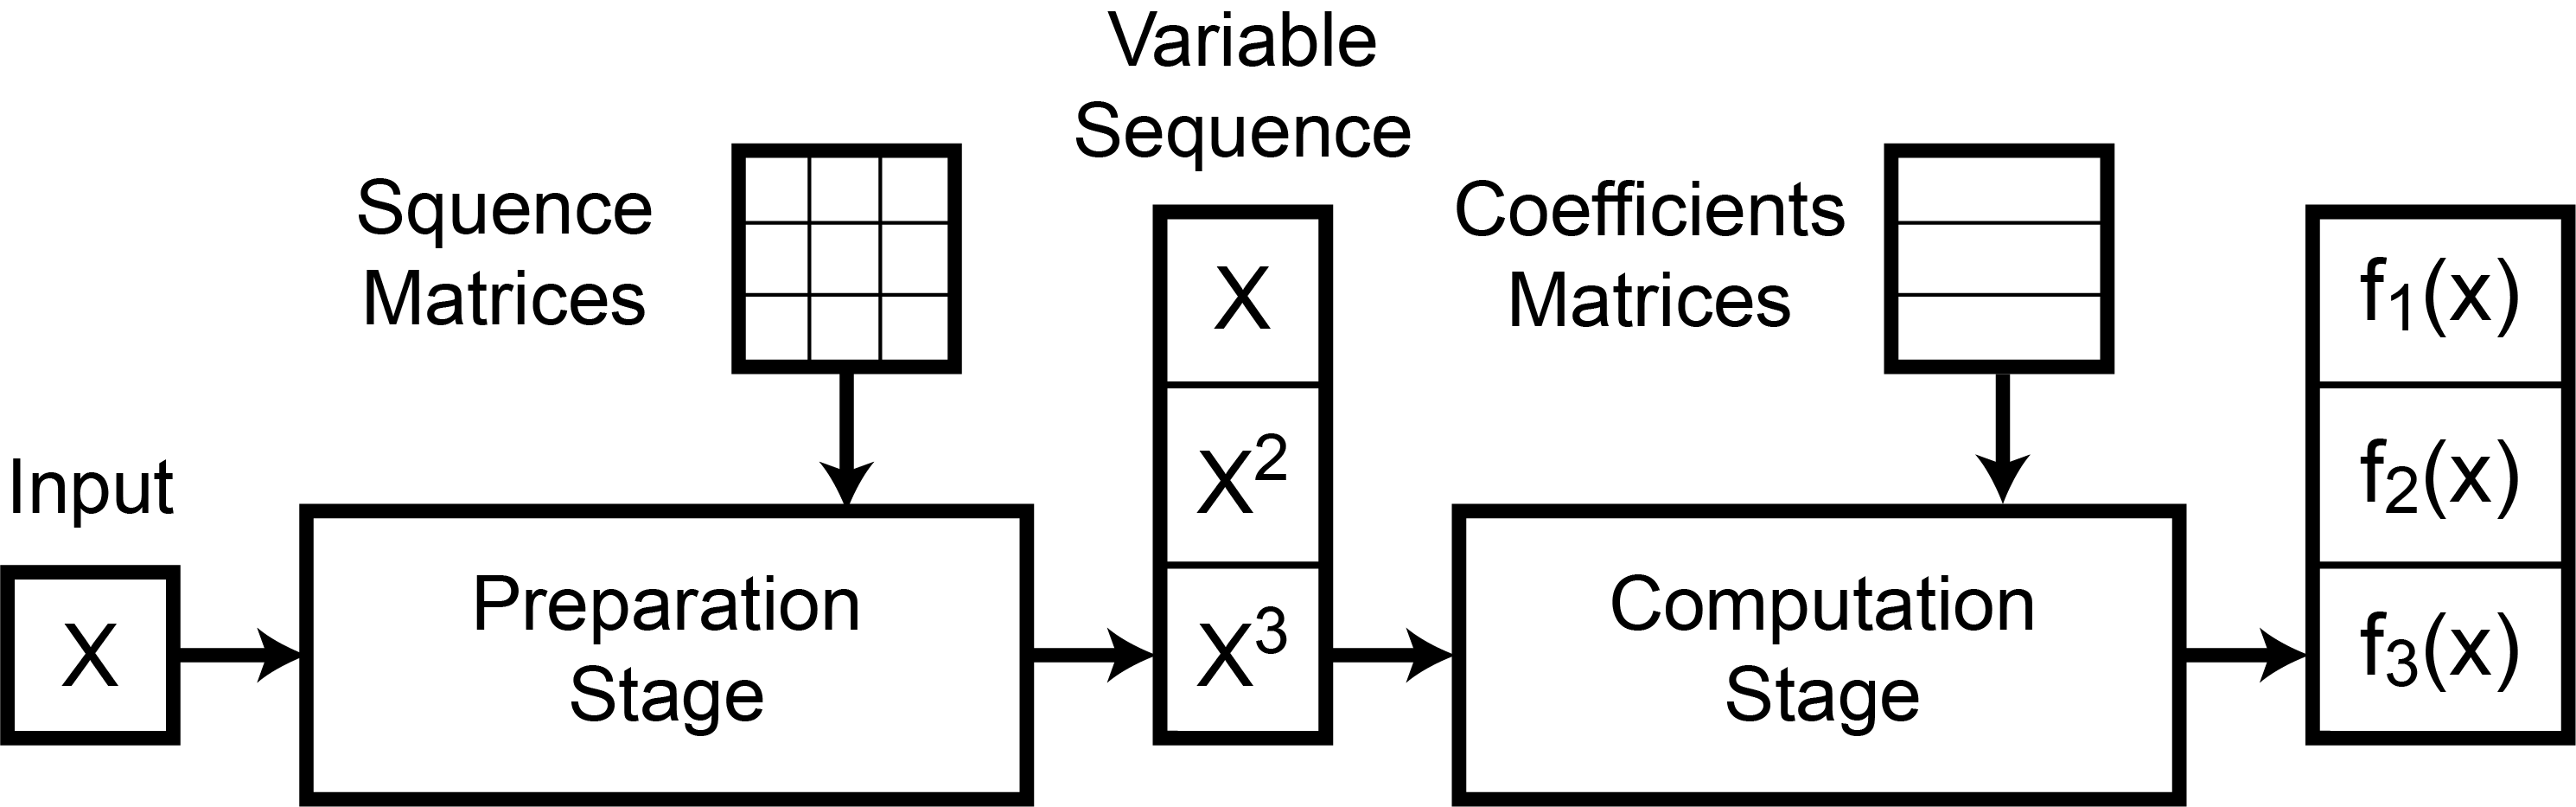
\includegraphics[scale=0.35]{figures/overview_2.png}}
    \caption{An overview of Cube-fx Algorithm for a single input}
    \label{fig:overview}
    \end{figure}

\subsection{Computation Stage}

The computation stage is mainly a matrix multiplication, shown in Eq. \ref{eq:comp_mat}, where $m$ is the number of inputs $(x_1, x_2, ..., x_m)$, $k$ is the order number, and $j$ is the number of evaluated functions. The left matrix of the matrix multiplication is a matrix of the Variable Sequence $(x, x^2, x^3, ...)$, which is built from the inputs and listed in the row-major order. The right matrix is the Coefficients Matrix, which is expanded from multiple functions $(f_a, f_b, ..., f_j)$ to $k$ order and listed in the column-major order. For each evaluated function $(f_a, f_b, ..., f_j)$, the coefficients of Taylor polynomials are $(a_1, a_2, ..., a_k)$, $(b_1, b_2, ..., b_k)$, $...$, $(j_1, j_2, ..., j_k)$. In this way, each element of the result matrix is a function evaluation result based on its related Taylor polynomial. For the example of $f_t(x)$ in the lower part of Eq. \ref{eq:comp_mat}, which is expanded at point $p$, the elements in column $t$ of the result matrix are the evaluation results of $f_t(x)$ with inputs from $(x_1, x_2, ..., x_m)$ and the coefficients $(t_1, t_2, ..., t_k)$. Therefore, the computation stage evaluates $(m \times j)$ Taylor polynomials in one step with the Matrix MACs.

\begin{equation}
    \label{eq:comp_mat}
    \begin{aligned}
    \setlength{\arraycolsep}{1.5pt}
        \begin{bmatrix} 
            x_1    & x_1^2  &   \dots   & x_1^k  \\
            x_2    & x_2^2  &   \dots   & x_2^k  \\
            \vdots &        & \ddots    & \vdots \\
            x_m    & x_m^2  &   \dots   & x_m^k  
        \end{bmatrix}
        \begin{bmatrix} 
            a_1    & b_1    &   \dots   & j_1 \\
            a_2    & b_2    &   \dots   & j_2  \\
            \vdots &        & \ddots    & \vdots \\
            a_k    & b_k    &   \dots   & j_k  
        \end{bmatrix}
        \approx
        \begin{bmatrix}
            f_{a}(x_1)  &     \dots   & f_{j}(x_1)    \\
            f_{a}(x_2)  &     \dots   & f_{j}(x_2)    \\
            \vdots      & \ddots    & \vdots        \\
            f_{a}(x_m)  &   \dots   & f_{j}(x_m)
        \end{bmatrix} \\
        f_t(x) = \sum_{s = 0}^{k}\frac{f_t^{(s)}(p)}{s!}(x - p)^s + o[(x - p) ^ k] \\
        \approx t_1x + t_2x^2 + \dots + t_kx^k
    \end{aligned}
    \end{equation}

Since the evaluated functions are chosen before launching the kernel, the values of the right matrix, the Coefficient Matrix, are predetermined and constant. Therefore, we consider the Coefficient Matrix a read-only memory segment that can be directly written in kernel codes. On the other hand, the data layout requirement of the left matrix, the Variable Sequence Matrix, is more stringent. For most of the AI processors, the left matrix of the Matrix MACs adopts the row-major, including Nvidia GPUs with tensor cores \cite{DBLP:conf/ipps/00020C20}, Cambricon MLUs \cite{cambricon}, and Huawei Ascend AI processors in this paper \cite{DBLP:conf/hotchips/LiaoTXZ19}. With the right matrix in column-major, the design can significantly improve the efficiency of matrix multiplications. Then, for a variable sequence $(x_{i}, x_{i}^2,  x_{i}^3, ...)$ mapped by the input $x_{i}$ in the Variable Sequence Matrix, as shown in \ref{eq:comp_mat}, it should be stored contiguously in the memory. In other words, after the preparation stage, the data at the memory address $x_{i + 1}$ in the kernel inputs should be moved to $x_{i + k}$ with its powers at $(x_{i + k + 1}, x_{i + k + 2}, ...)$. Then, its neighbor, data at $x_{i + 2}$, should be moved to $x_{i + 2k}$ with its powers at $(x_{i + 2k + 1}, x_{i + 2k + 2}, ...)$. Without a built-in vectorized \textit{scatter} instruction, the scattering process could only be done by weak scalar operations for each input $x_{i}$, which significantly ruins the kernel performance of the AI processors. Therefore, the primary objective of the preparation stage is to complete the scattering process with the Matrix MACs instead of the vector or scalar units.

\subsection{Preparation Stage}

\begin{equation}
    \label{eq:power}
    \begin{aligned}
        e^{k \ln v} = e^{\ln v^k} = v^k
    \end{aligned}
    \end{equation}

The preparation stage of Cube-fx is based on two mathematical formulas. The first combines the logarithmic power law and the logarithmic definition, given in Eq. \ref{eq:power}, where $k$ is a constant, $v \in \mathbb{R}$, converting the product to power.

\begin{equation}
    \label{eq:spec_mat}
    \begin{aligned}
        \setlength{\arraycolsep}{2pt}
        \begin{bmatrix} 
            \ln v_{1, 1}    & \dots     & \ln v_{1, s}  \\
            \vdots      & \ddots    & \vdots    \\
            \ln v_{m, 1}    & \dots     & \ln v_{m, s} 
        \end{bmatrix}
        \cdot
        mat
        =
        \begin{bmatrix}
            \ln {v_{1, i_0}}^{k_1} & \dots     & \ln {v_{1, i_0}}^{k_{j_0}}  \\
            \vdots          & \ddots    & \vdots                \\
            \ln {v_{m, i_0}}^{k_1}  & \dots    & \ln {v_{m, i_0}}^{k_{j_0}}  \\
        \end{bmatrix} \\
        mat = (b_{i, j}) \in \mathbb{F}^{s \times j_0}, 
        b_{i, j} = \left\{
                        \begin{array}{lc}
                            0, i \neq i_{0} \\
                            k_j, i = i_{0}
                        \end{array}
                    \right.
    \end{aligned}
    \end{equation}

The second formula is a special case of matrix multiplications, given in Eq. \ref{eq:spec_mat}, where the left matrix is an input matrix of $(m \times s)$, $p_{i, j} \in \mathbb{R}$, the right matrix $mat$ is a matrix of $(s \times j_0)$, $k_{j} \in \mathbb{R}$. Except for a non-zero vector $(k_1, k_2, \dots, k_{j_0})$ at the row $i_0$, all other elements $b_{i, j}$ of $mat$ are $0$. Therefore, the matrix multiplication, shown as Eq. \ref{eq:spec_mat}, computes the products of the column $i_0$ of the left matrix $(\ln v_{1, i_0}, \ln v_{2, i_0}, ..., \ln v_{m, i_0})^{T}$, the exponents of Eq. \ref{eq:power}, and the row $i_0$ of the right matrix $(k_1, k_2, ..., k_{j_0})$ to form a full result matrix. Therefore, the required variable sequences are computed with an extra logarithmic operation.

\begin{algorithm}[tb]
    \caption{Preparation stage of Cube-fx}
    \setlength{\arraycolsep}{1.2pt}
    \label{alg:prepare}
    \SetKwInOut{Input}{Input}
    \SetKwInOut{Output}{Output}
        
    \Input{
        input 1D array \textbf{V} of the size $N$ \\
    }
    \Output{
        result sequences \textbf{Sq} of the size $(N \times k)$
    }
    
    \BlankLine
    \BlankLine
    
    $mat[s] \leftarrow 
            \underbrace{            
                \begin{bmatrix} 1 & 2 & 3 & \dots & k   \\ 
                                0 & 0 & 0 & \dots & 0   \\
                                  &   &   & \dots &     \\ 
                                0 & 0 & 0 & \dots & 0 
                \end{bmatrix}
                \dots
                \begin{bmatrix}   &   &   & \dots &     \\ 
                                1 & 2 & 3 & \dots & k   \\ 
                                  &   &   & \dots &     \\ 
                                0 & 0 & 0 & \dots & 0 
                \end{bmatrix}
                \dots
                \begin{bmatrix} 0 & 0 & 0 & \dots & 0   \\ 
                                0 & 0 & 0 & \dots & 0   \\
                                  &   &   & \dots &     \\ 
                                1 & 2 & 3 & \dots & k
                \end{bmatrix}
            }_{An\ s-array\ of\ (s \times k)\ matrices}
    $ \\
    \BlankLine
    \BlankLine
    $\textbf{V}_{ln} \leftarrow \textbf{ln}(\textbf{V})$ \\
    $\textbf{V}_{mat} \leftarrow$ reinterpret $\textbf{V}_{ln}$ as a $(N / s) \times s$ matrix \\
    \For{$idx \leftarrow 0$ \KwTo $s$} {
        $\textbf{Sq}_{mat}[idx] \leftarrow \textbf{V}_{mat} \cdot mat[idx]$ \\
        $\textbf{Sq}_{ln}[idx] \leftarrow$ reinterpret $\textbf{Sq}_{mat}[idx]$ as an 1D array \\
        $\textbf{Sq}[idx] \leftarrow $ \textbf{exp}($\textbf{Sq}_{ln}[idx]$)
    }
    \Return \textbf{Sq}
\end{algorithm}

Based on the two formulas, Alg. \ref{alg:prepare} presents the preparation stage of Cube-fx, where we consider the shape of the Matrix MACs is $(s \times s)$. In the beginning, Alg. \ref{alg:prepare} initializes an $s$-element array of $(s \times k)$ Sequence Matrices $mat[s]$, as we described in Eq. \ref{eq:spec_mat}. For the $idx$-th Sequence Matrix $mat[idx]$, the non-zero row is at row $idx$, whose value is an increasing vector $(1, 2, \dots, k)$. Therefore, for each row $idx$ of the $(s \times s)$ Matrix MACs, we construct a unique Sequence Matrix with a non-zero vector at that row. Then, Alg. \ref{alg:prepare} computes the logarithmic results $\textbf{V}_{ln}$ of the input $\textbf{V}$ with the built-in vectorized operation. The logarithmic results are reinterpreted as an $(\frac{N}{s} \times s)$ matrix $\textbf{V}_{mat}$ and transferred to the Matrix MAC. 
At the mathematical level, the reinterpretation constructs the left matrix in Eq. \ref{eq:spec_mat}, where $m = \frac{N}{s}$. At the system level, Huawei Ascend processors adopt a row-major order for the $(16 \times 16)$ left matrix of the basic matrix multiplication as discussed in Sec. \ref{sec:2.1}. Therefore, the continuous memory segment $\textbf{V}_{ln}$ requires no additional data layout conversion, as it is inherently indexed in Z-order as an $(\frac{N}{s} \times s)$ through a single data transfer operation to the Matrix MAC.
% Especially, the reinterpretation needs no physical data layout conversion but only from the logical view. 

\begin{figure}[t]
    \centering{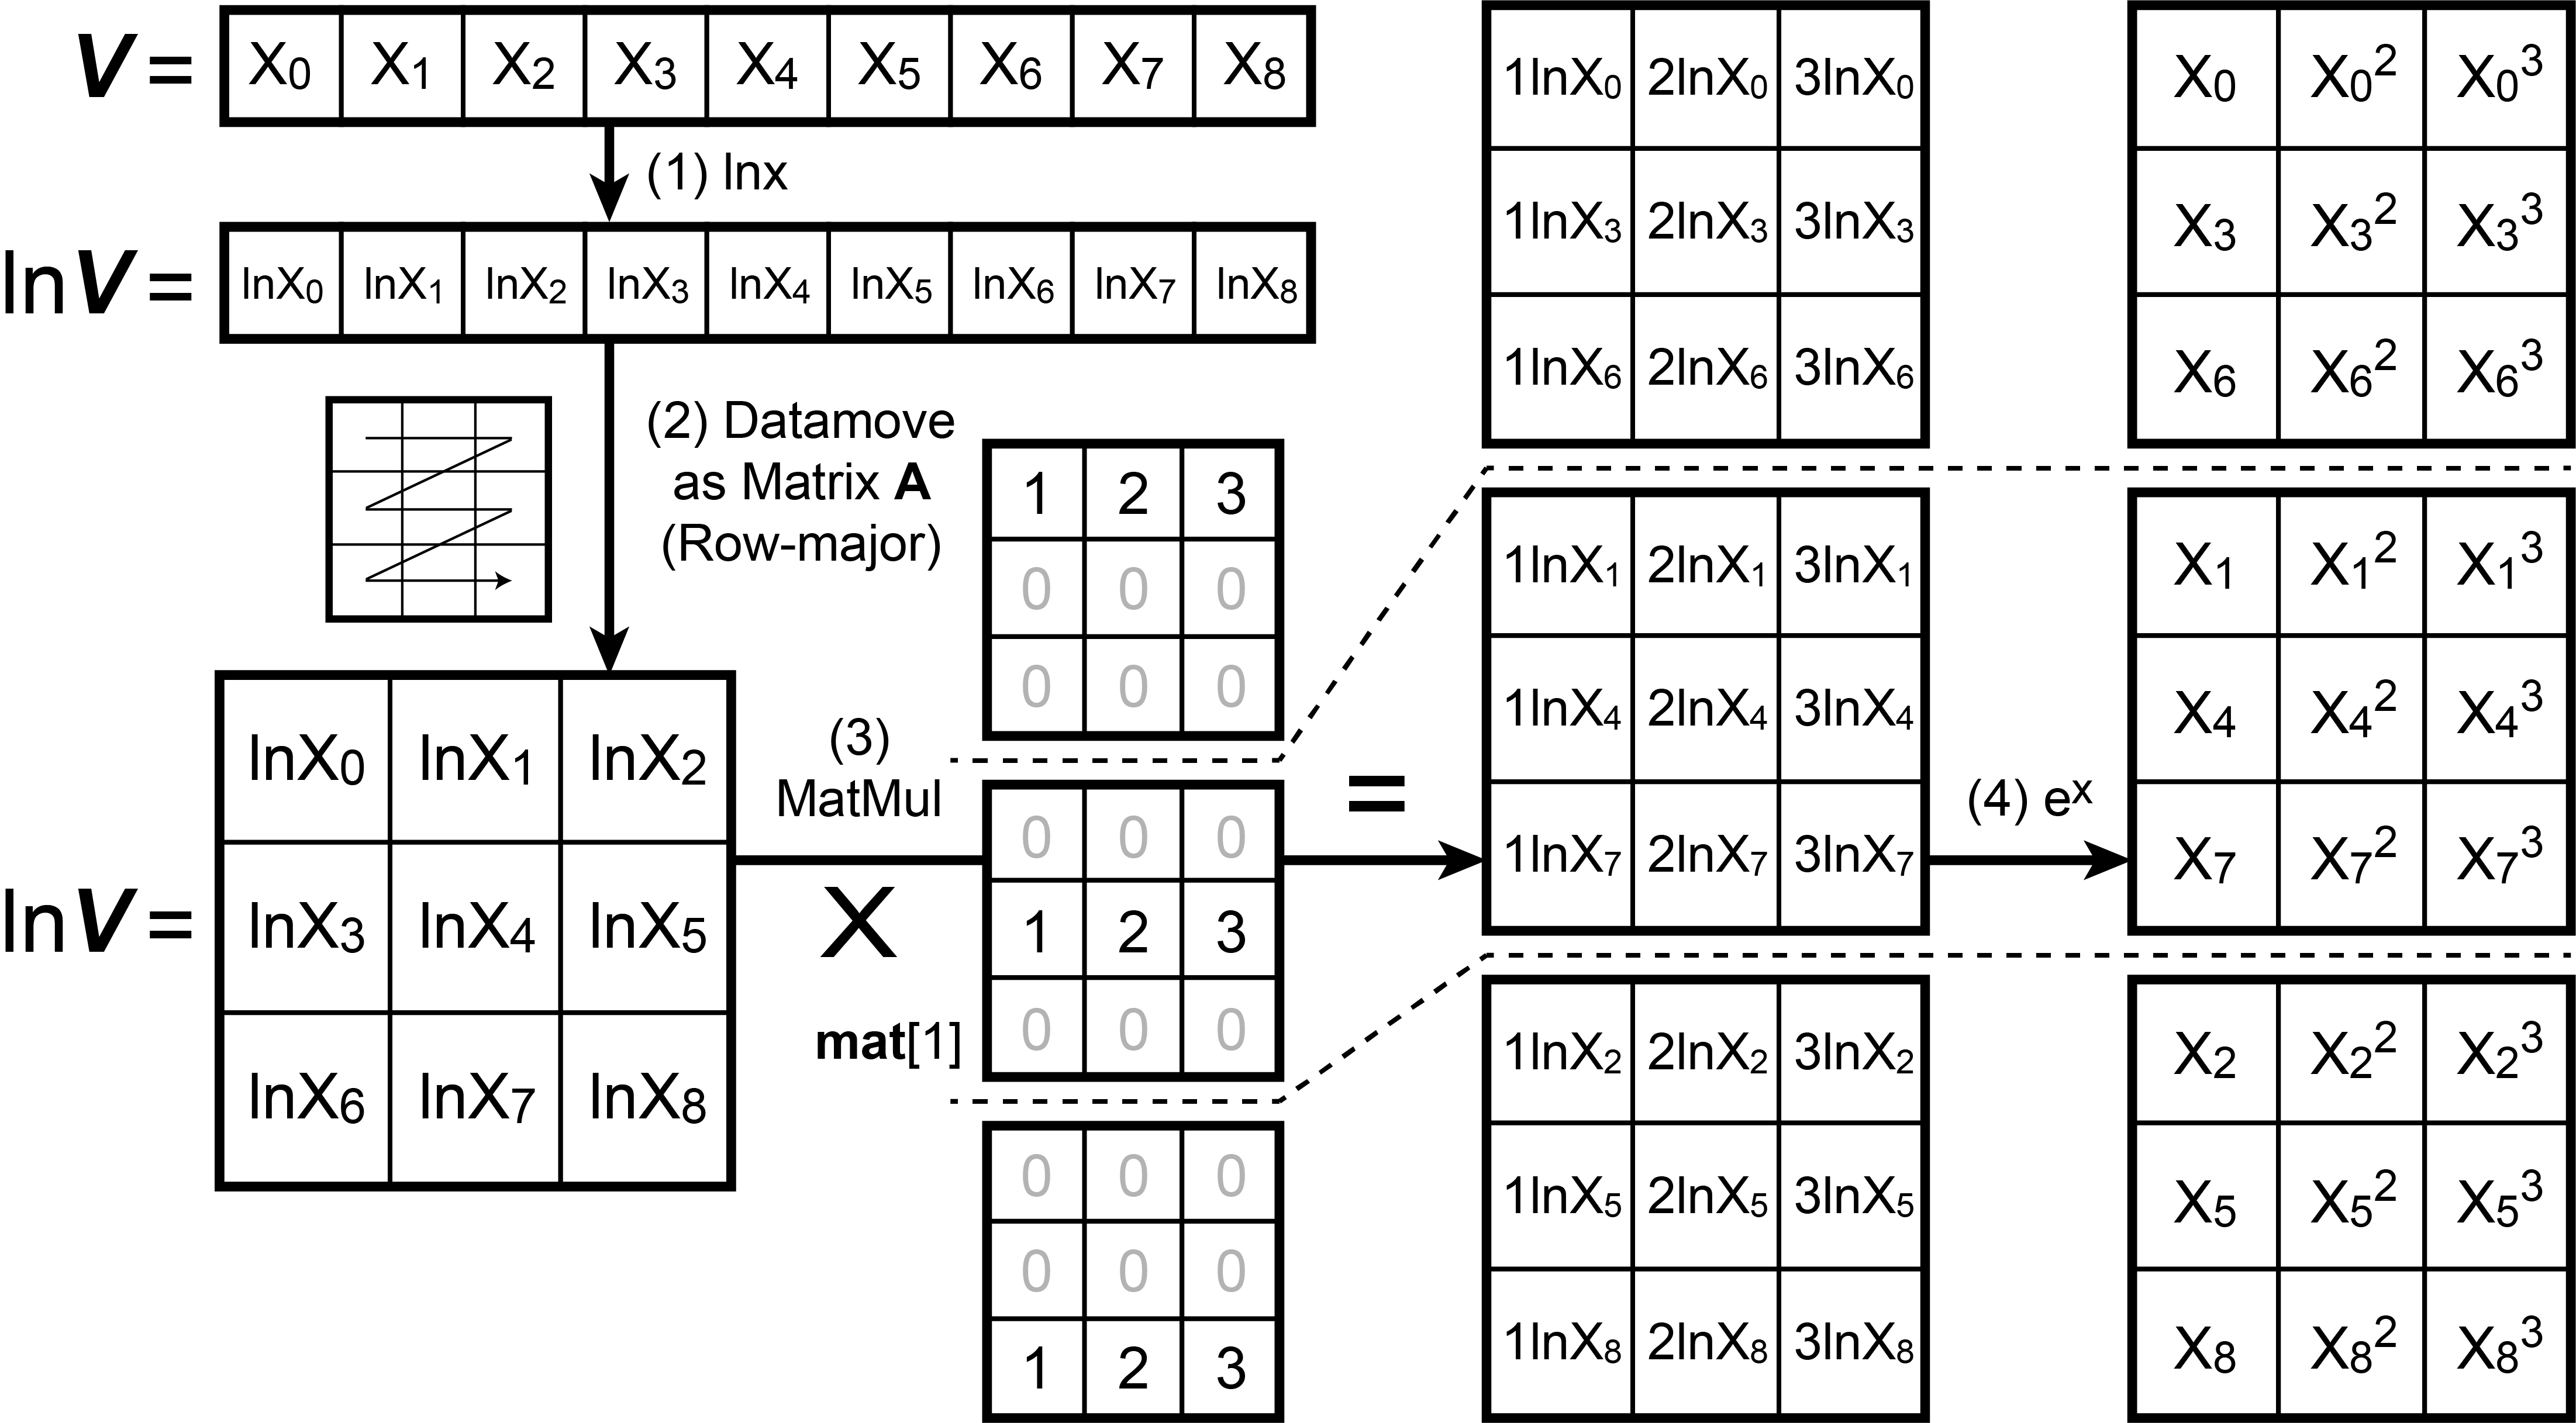
\includegraphics[scale=0.32]{figures/trans_ln.png}}
    \caption{An example for 9 inputs with $3 \times 3$ Matrix MACs}
    \label{fig:trans_ln}
    \end{figure}

The next step is the central step of the preparation stage, which is an $s$-step loop. In the loop step $idx$, the logarithmic inputs $\textbf{V}_{mat}$ take matrix multiplications with the Sequence Matrix $mat[idx]$. As discussed in Eq. \ref{eq:spec_mat}, the $idx$-th matrix multiplication generates the $(\frac{N}{s} \times s)$ Variable Sequence matrix for the column $idx$ of the logarithmic inputs. For the example of the second matrix multiplication in Fig. \ref{fig:trans_ln}, the non-zero row of the second Sequence Matrix $mat[1]$ is at the second row $mat[1][1, :]$. Therefore, the result matrix is formed by the product of the second column of the logarithmic inputs $\textbf{V}_{mat}[:, 1]$ and the increasing vector $(1, 2, \dots, k)$. Since the logarithmic results are shaped as $(\frac{N}{s} \times s)$, $s$ columns need $s$ loop steps and the Sequence Matrice in total.

After the matrix multiplication in each loop step, the preparation stage applies an exponential function to the result matrices, which is reinterpreted as an array. As shown in Eq. \ref{eq:power}, it restores the logarithmic product results $\textbf{Sq}_{ln}$ to the original power results. Finally, the preparation stage completes the construction of the Variable Sequence, which perfectly meets the data layout requirement of the computation stage. In addition, although the results are currently shaped as an array, similar to $\textbf{V}_{ln}$ without extra operations, they can be directly passed to the computation stage as $(\frac{N}{s} \times k)$ matrices.

\begin{figure}[t]
    \centering{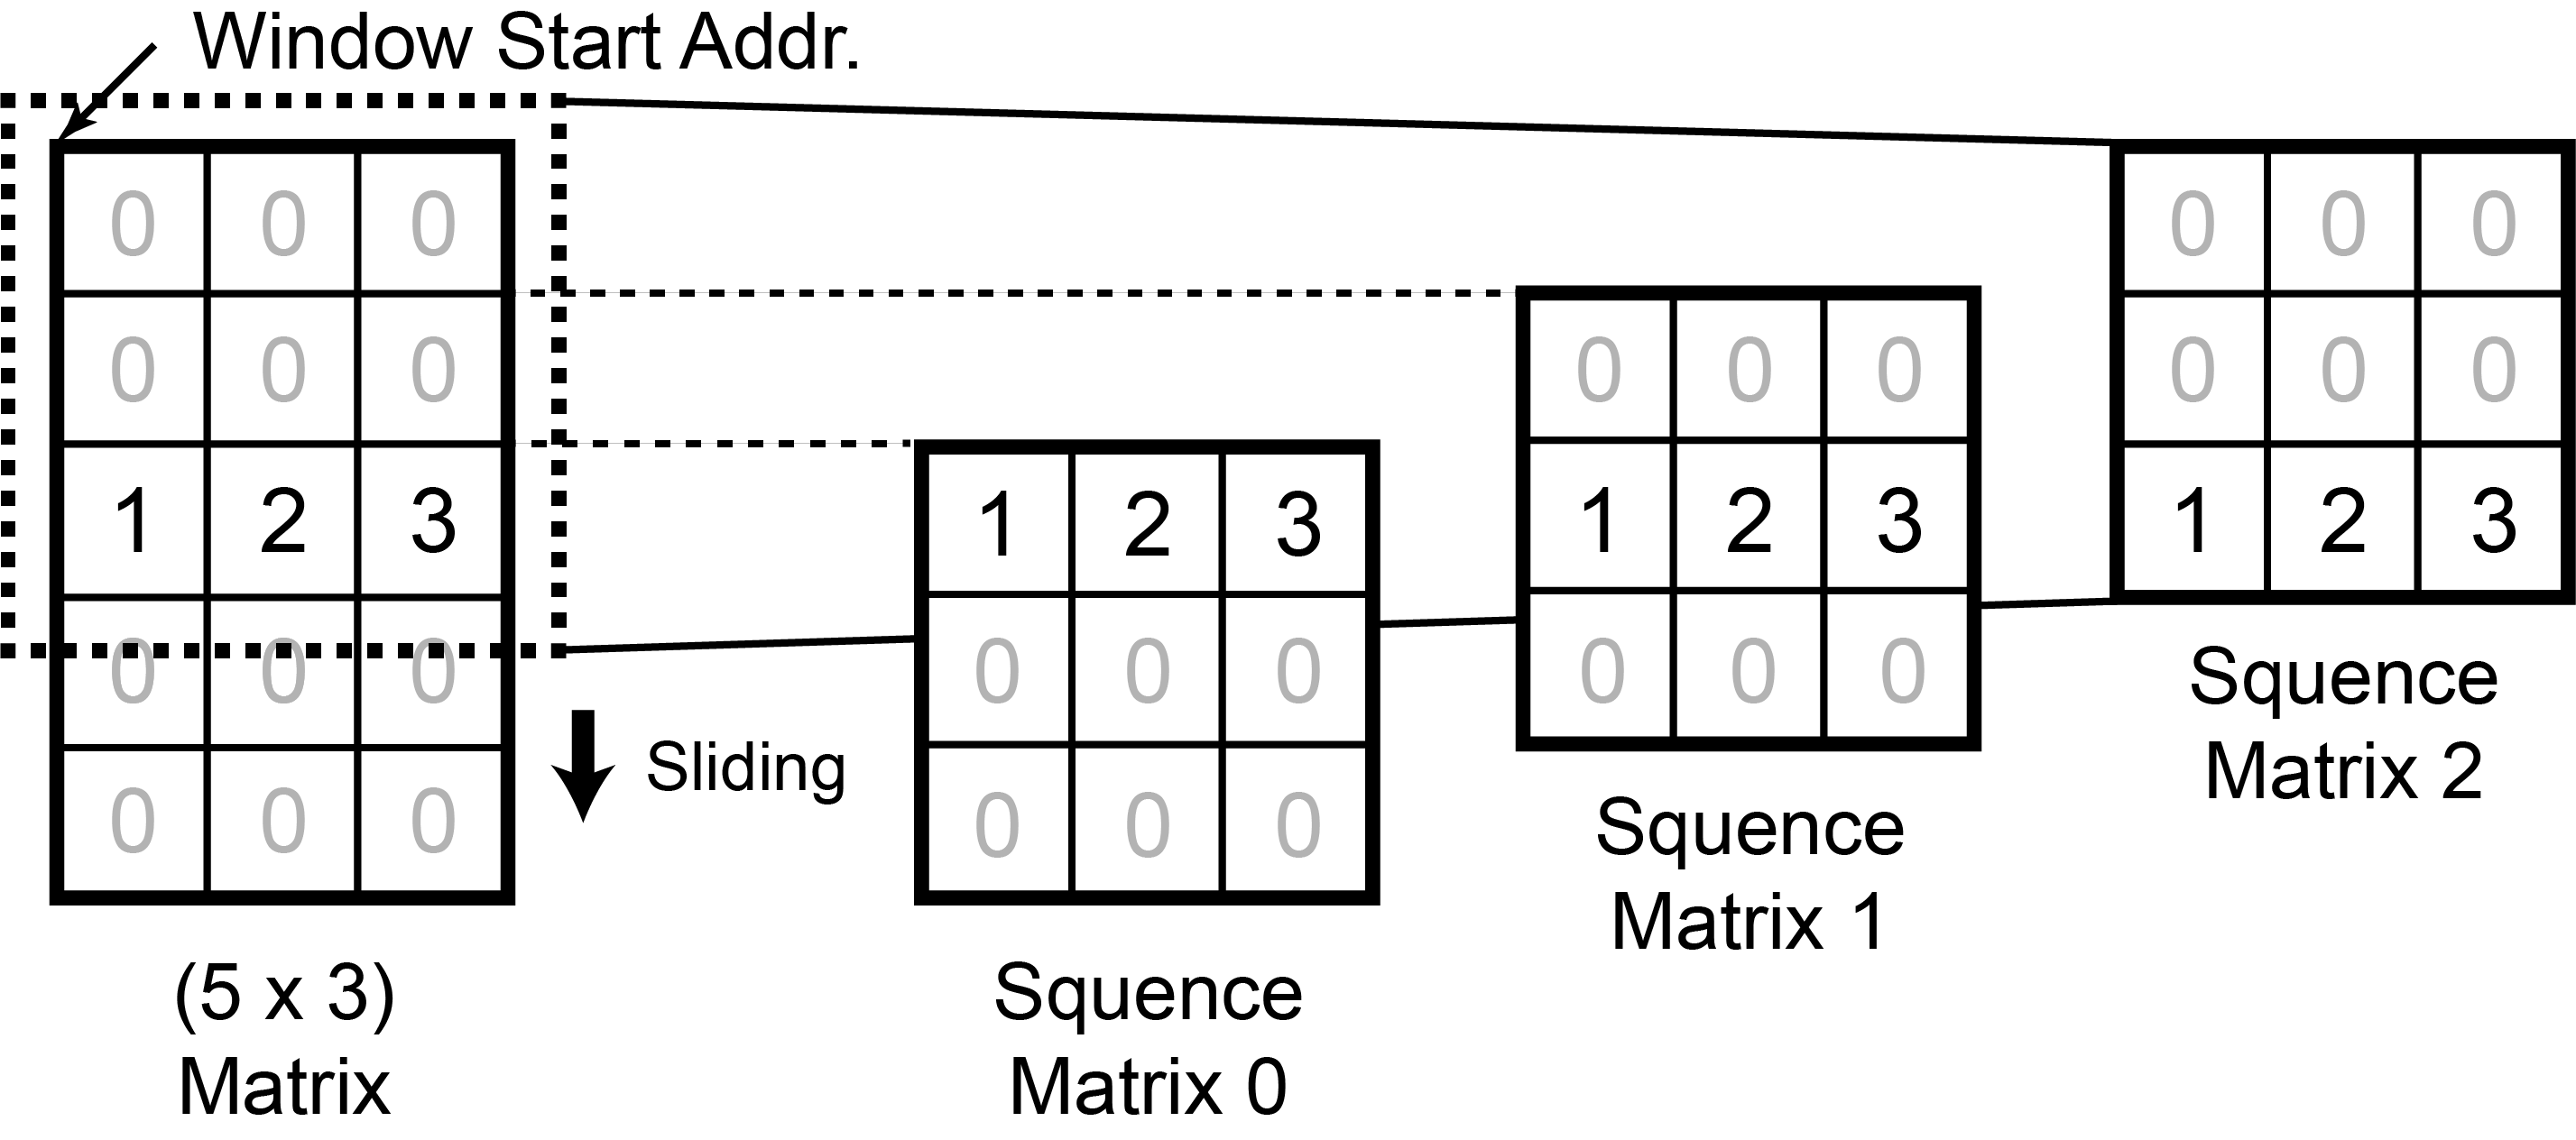
\includegraphics[scale=0.35]{figures/window.png}}
    \caption{An example for the sliding window for 9 inputs with $3 \times 3$ Matrix MACs}
    \label{fig:window}
    \end{figure}

The time complexity of the preparation stage is $O(Nk) + O(Nk / s^2)$ for sequential execution, where $N$ is the size of input data, $k$ is the order number of Taylor expansion, and $s$ is the side length of the Matrix MACs. The first part $O(Nk)$ is the time complexity of the vectorized operations, which equals that of Horner's Method. The second part $O(Nk / s^2)$ is the time complexity of the matrix multiplications on the Matrix MACs. Theoretically, the execution time of the preparation stage is slightly longer than Horner's Method for a single-function evaluation. In detail, the number of vectorized operations of the preparation stage is $Nk + N$, while that of Horner's Method is $2Nk$. Therefore, although the vectorized operations of Cube-fx are $exp$ and $ln$, the preparation stage still performs similarly to Horner's Method. In addition, the execution of the Matrix MACs and Vector Units can be scheduled concurrently. In theory, the longer execution can entirely hide the execution of the other. Therefore, the concurrent time complexity can be reduced to $max(O(Nk), O(Nk / s^2))$ in the best situation. We will describe the concurrent execution in the following subsection. As a result, the time complexity of the preparation stage is acceptable since it is built for multiple functions instead of only one function in the later computation stage. 

For the space complexity, the extra memory needed by the preparation stage is $O(ks^2)$, which stores the preparation matrices. However, a sliding window policy can reduce the space complexity to $O(ks)$, which allocates $((2/s - 1) \times n)$ matrix. As shown in \ref{fig:window}, the non-vector is at the second row, while other rows are filled with $0$. Therefore, when the $(3 \times 3)$ windows slide down from row $0$ to row $2$, the three required Sequence Matrices are offered respectively.

\subsection{Concurrent Execution \label{sec:3.3}}

Since Cube-fx executes on the Matrix MACs and vectorized units, a naive sequential implementation could keep one unit idle while the other is busy, as well as the related data movement. Therefore, this subsection demonstrates a concurrent implementation on Ascend 910B processors.

\begin{algorithm}[tbp]
    \caption{Concurrent Cube-fx on Ascend 910B}
    \setlength{\arraycolsep}{1.2pt}
    \label{alg:concurrent}
    \SetKwInOut{Input}{Input}
    \SetKwInOut{Output}{Output}
    \SetKwBlock{VecBlock}{Vec:}{}
    \SetKwBlock{CubeBlock}{Cube:}{}
        
    \Input{
        input 1D array \textbf{$V$} of the size $N$ \\
        input 2D array \textbf{C} of the size $(k \times j)$
    }
    \Output{
        results \textbf{Res} of the size $(N \times j)$
    }

    \VecBlock {
        \nonl$\textbf{$V_{ln}$} \leftarrow \textbf{ln}(\textbf{$V$})$ \\
    } 
    \nonl\CubeBlock {
        \nonl$mat[s] \leftarrow Array\ of\ (s \times k)\ matrices$ 
    }

    \CubeBlock {
        \nonl$\textbf{V}_{mat} \leftarrow$ reinterpret $\textbf{V}_{ln}$ as a $(N / s) \times s$ matrix \\
        \nonl\For{$idx \leftarrow 0$ \KwTo $s / 2$} {
            \nonl$\textbf{Sq}_{mat}[idx] \leftarrow \textbf{V}_{mat} \cdot mat[idx]$
        }
    }

    \VecBlock {
        \nonl\For{$idx \leftarrow 0$ \KwTo $s / 2$} {
            \nonl$\textbf{Sq}_{ln}[idx] \leftarrow$ reinterpret $\textbf{Sq}_{mat}[idx]$ as an 1D array \\
            \nonl$\textbf{Sq}[idx] \leftarrow $ \textbf{exp}($\textbf{Sq}_{ln}[idx]$)
        }
    }
    \nonl\CubeBlock {
        \nonl\For{$idx \leftarrow s / 2$ \KwTo $s$} {
            \nonl$\textbf{Sq}_{mat}[idx] \leftarrow \textbf{V}_{mat} \cdot mat[idx]$ \\
        }
    }

    \VecBlock {
        \nonl\For{$idx \leftarrow s / 2$ \KwTo $s$} {
            \nonl$\textbf{Sq}_{ln}[idx] \leftarrow$ reinterpret $\textbf{Sq}_{mat}[idx]$ as an 1D array \\
            \nonl$\textbf{Sq}[idx] \leftarrow $ \textbf{exp}($\textbf{Sq}_{ln}[idx]$)
        }
    }
    \nonl\CubeBlock {
        \nonl$\textbf{Sq}_{mat_{0}} \leftarrow$ reinterpret $\textbf{Sq}[0:N/2][:]$ as a $(N / 2) \times k$ matrix \\
        \nonl$\textbf{Res}[0:N/2][:] \leftarrow \textbf{Sq}_{mat_{0}} \cdot \textbf{C} $
    }

    \CubeBlock {
        \nonl$\textbf{Sq}_{mat_{1}} \leftarrow$ reinterpret $\textbf{Sq}[N/2:N][:]$ as a $(N / 2) \times k$ matrix \\
        \nonl$\textbf{Res}[N/2:N][:] \leftarrow \textbf{Sq}_{mat_{1}} \cdot \textbf{C} $
    }
    \Return \textbf{Res}
\end{algorithm}

To achieve concurrent execution on Ascend 910B processors, a technology named Double Buffer (or Ping Pong Buffer \cite{DBLP:conf/infocom/JooM98}) is used. Given an algorithm, we first split the source codes into the parts of Cube Units and Vector Units and mark the continuous segments with two units alternately appearing. Then, we cut the inputs of the marked segments into several pieces and then execute the pieces one by one to manually create a pipeline. The key is that while executing the second piece of the first part on one unit (Cube Unit), the first piece of the second part, which follows the first part of codes, is also started on the other unit (Vector Unit). As given in Alg. \ref{alg:concurrent}, each step contains the concurrent operations on two units (\textbf{Cube} for Cube Units and \textbf{Vec} for Vector Units).
As shown in Fig. \ref{fig:dav}(b), Cube Units and Vector Units are separately located in Cube Cores and Vector Cores. While Cube Units compute the matrix multiplications as discussed in Sec. \ref{sec_1_2_2}, a Vector Unit computes a fixed-size and continuous data segment in the pattern of SIMD, similar to most vectorized units on CPUs \cite{avx}. In addition to the computation, Alg. \ref{alg:concurrent} also includes multiple data transfers through various data paths, connecting the global memory to the computation units.
An inter-core synchronization is required between every two steps. For the example of Alg. \ref{alg:concurrent}, in Step 2, the Cube Unit first computes the first segment of $\textbf{Sq}_{ln}$ between $0$ and $s / 2$. Then, in Step 3, the result is transferred to the Vector Unit for the later exponent computation. Meanwhile, the Cube Unit continues to compute the second segment of $\textbf{Sq}_{ln}$ between $s / 2$ and $s$. This way, the Cube and Vector Unit run concurrently in Step 3 and leave neither unit idle.


An inter-core synchronization is required between every two steps. For the example of Alg. \ref{alg:concurrent}, in Step 2, the Cube Unit first computes the first segment of $\textbf{Sq}_{ln}$ between $0$ and $s / 2$. Then, in Step 3, the result is transferred to the Vector Unit for the later exponent computation. Meanwhile, the Cube Unit continues to compute the second segment of $\textbf{Sq}_{ln}$ between $s / 2$ and $s$. This way, the Cube and Vector Unit run concurrently in Step 3 and leave neither unit idle.

Especially, it is noticed that in Step 2, 5 of Alg. \ref{alg:concurrent}, the Vector Units are still idle. Theoretically, by splitting the segments as small as possible, the idleness of the Vector Units could be ignorable. The concurrent time complexity is approaching $max(O(Nk), O(Nk / s^2))$ as we discussed. However, because of the slow inter-core binary semaphore, as discussed in Sec. \ref{sec_1_2_2}, too many synchronizations cause significant overheads, which would cancel the benefits from the concurrent execution. Therefore, on Ascend 910B processors, we only split the data into two segments. In contrast, on Ascend 310 processors, which have a much faster binary semaphore and lower synchronization overheads, we split the data into 16 segments in our implementation to reduce the idleness.

\section{Cube-fx for General Cases \label{sec:4}}

The last section introduces Cube-fx in the case where the Matrix MACs are always fully utilized. In this section, we extend the algorithm to more general instances where the Matrix MACs are not saturated ($k \mod s \neq 0$).

We first define a metric, Matrix MAC Count, to evaluate the scale of matrix multiplications. As mentioned in Sec. \ref{sec_1_2_2}, in one basic step, a Matrix MAC completes a fixed shape of matrix multiplication. Then, it accumulates the results from multiple steps as a whole matrix multiplication. Therefore, the Matrix MAC Count indicates how many basic fix-shaped matrix multiplications it takes for a Matrix MAC to finish a large matrix multiplication with the standard $O(n^3)$ block matrix multiplication algorithm. For example, for a Matrix MAC of the shape $(s \times s)$, the Matrix MAC Count of matrix multiplication of the shape $(m \times k \times n)$ is $(mkn / s^3)$. 

\subsection{Enhanced Mapping of Cube-fx}

\begin{figure}[t]
    \centering{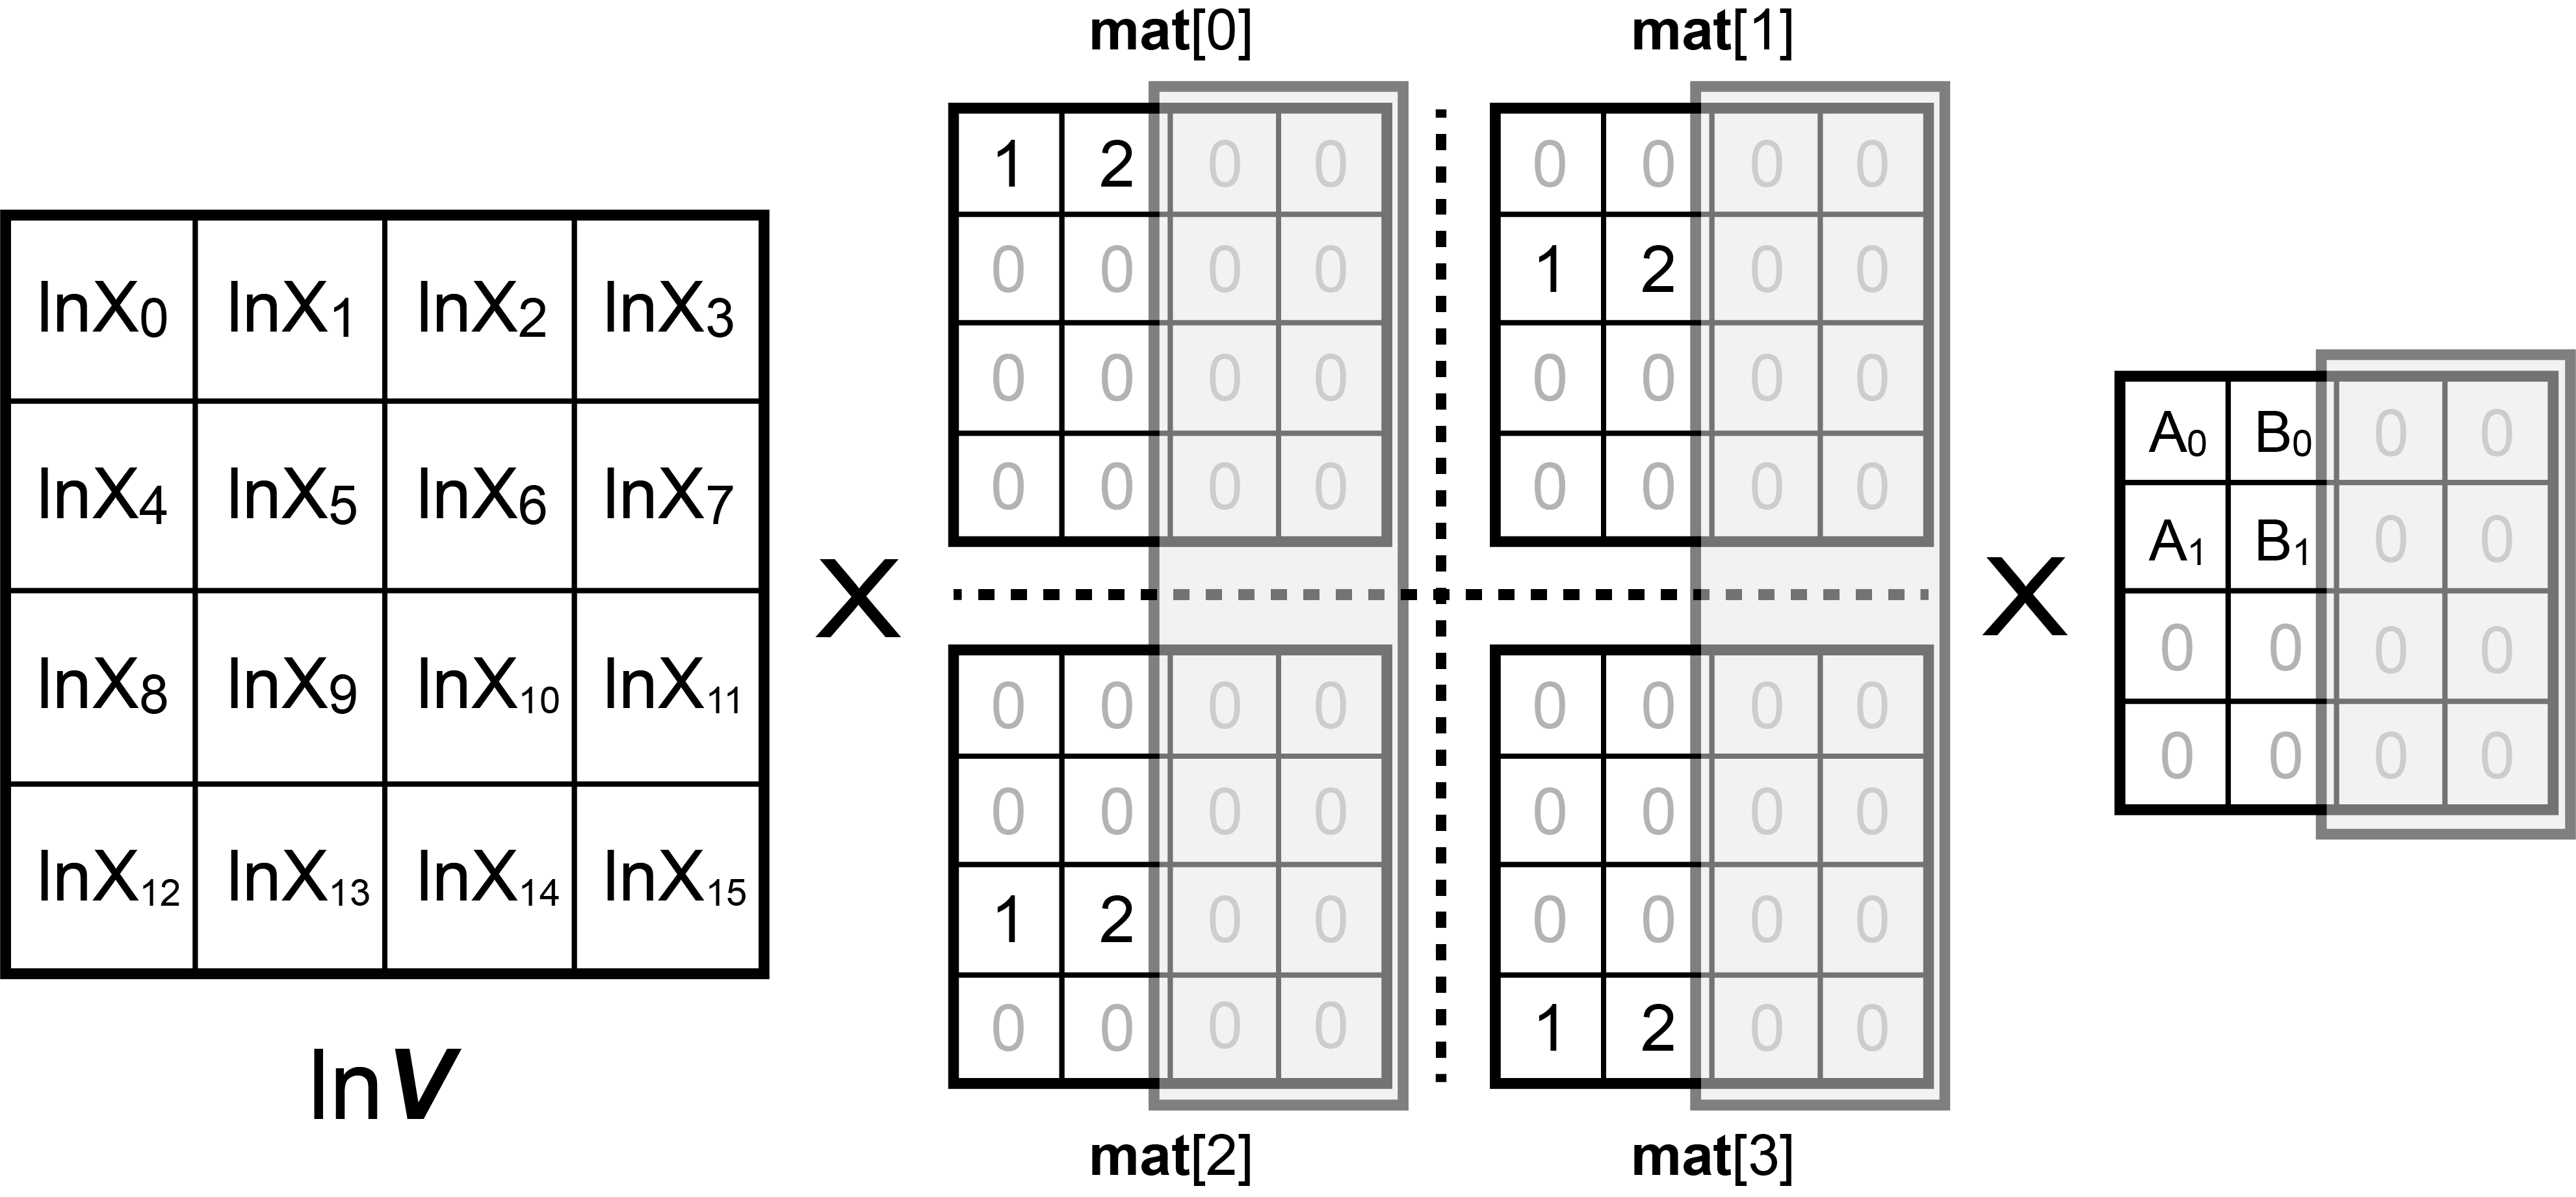
\includegraphics[scale=0.35]{figures/problem.png}}
    \caption{Naive Cube-fx where $s = 4, k = 2, j = 2$}
    \label{fig:problem}
    \end{figure}

Since the evaluation precision is not always the most significant target, the Taylor series's order requirement is flexible to improve efficiency with sight precision loss \cite{math}. Therefore, in these situations, the order number does not have to equal the slide length of the Matrix MACs. Fig. \ref{fig:problem} shows a naive application of Cube-fx where the order number is two, the side length is four, and the evaluated function number is two. In this case, we can easily observe that half of the Matrix MAC units we shade are full of zeros in the preparation and computation stages. Since all the units of the Matrix MACs must be utilized in each step of the matrix multiplication, the shaded units' computation power and results are wasted, which generates meaningless zeros.

\begin{figure}[t]
    \centering{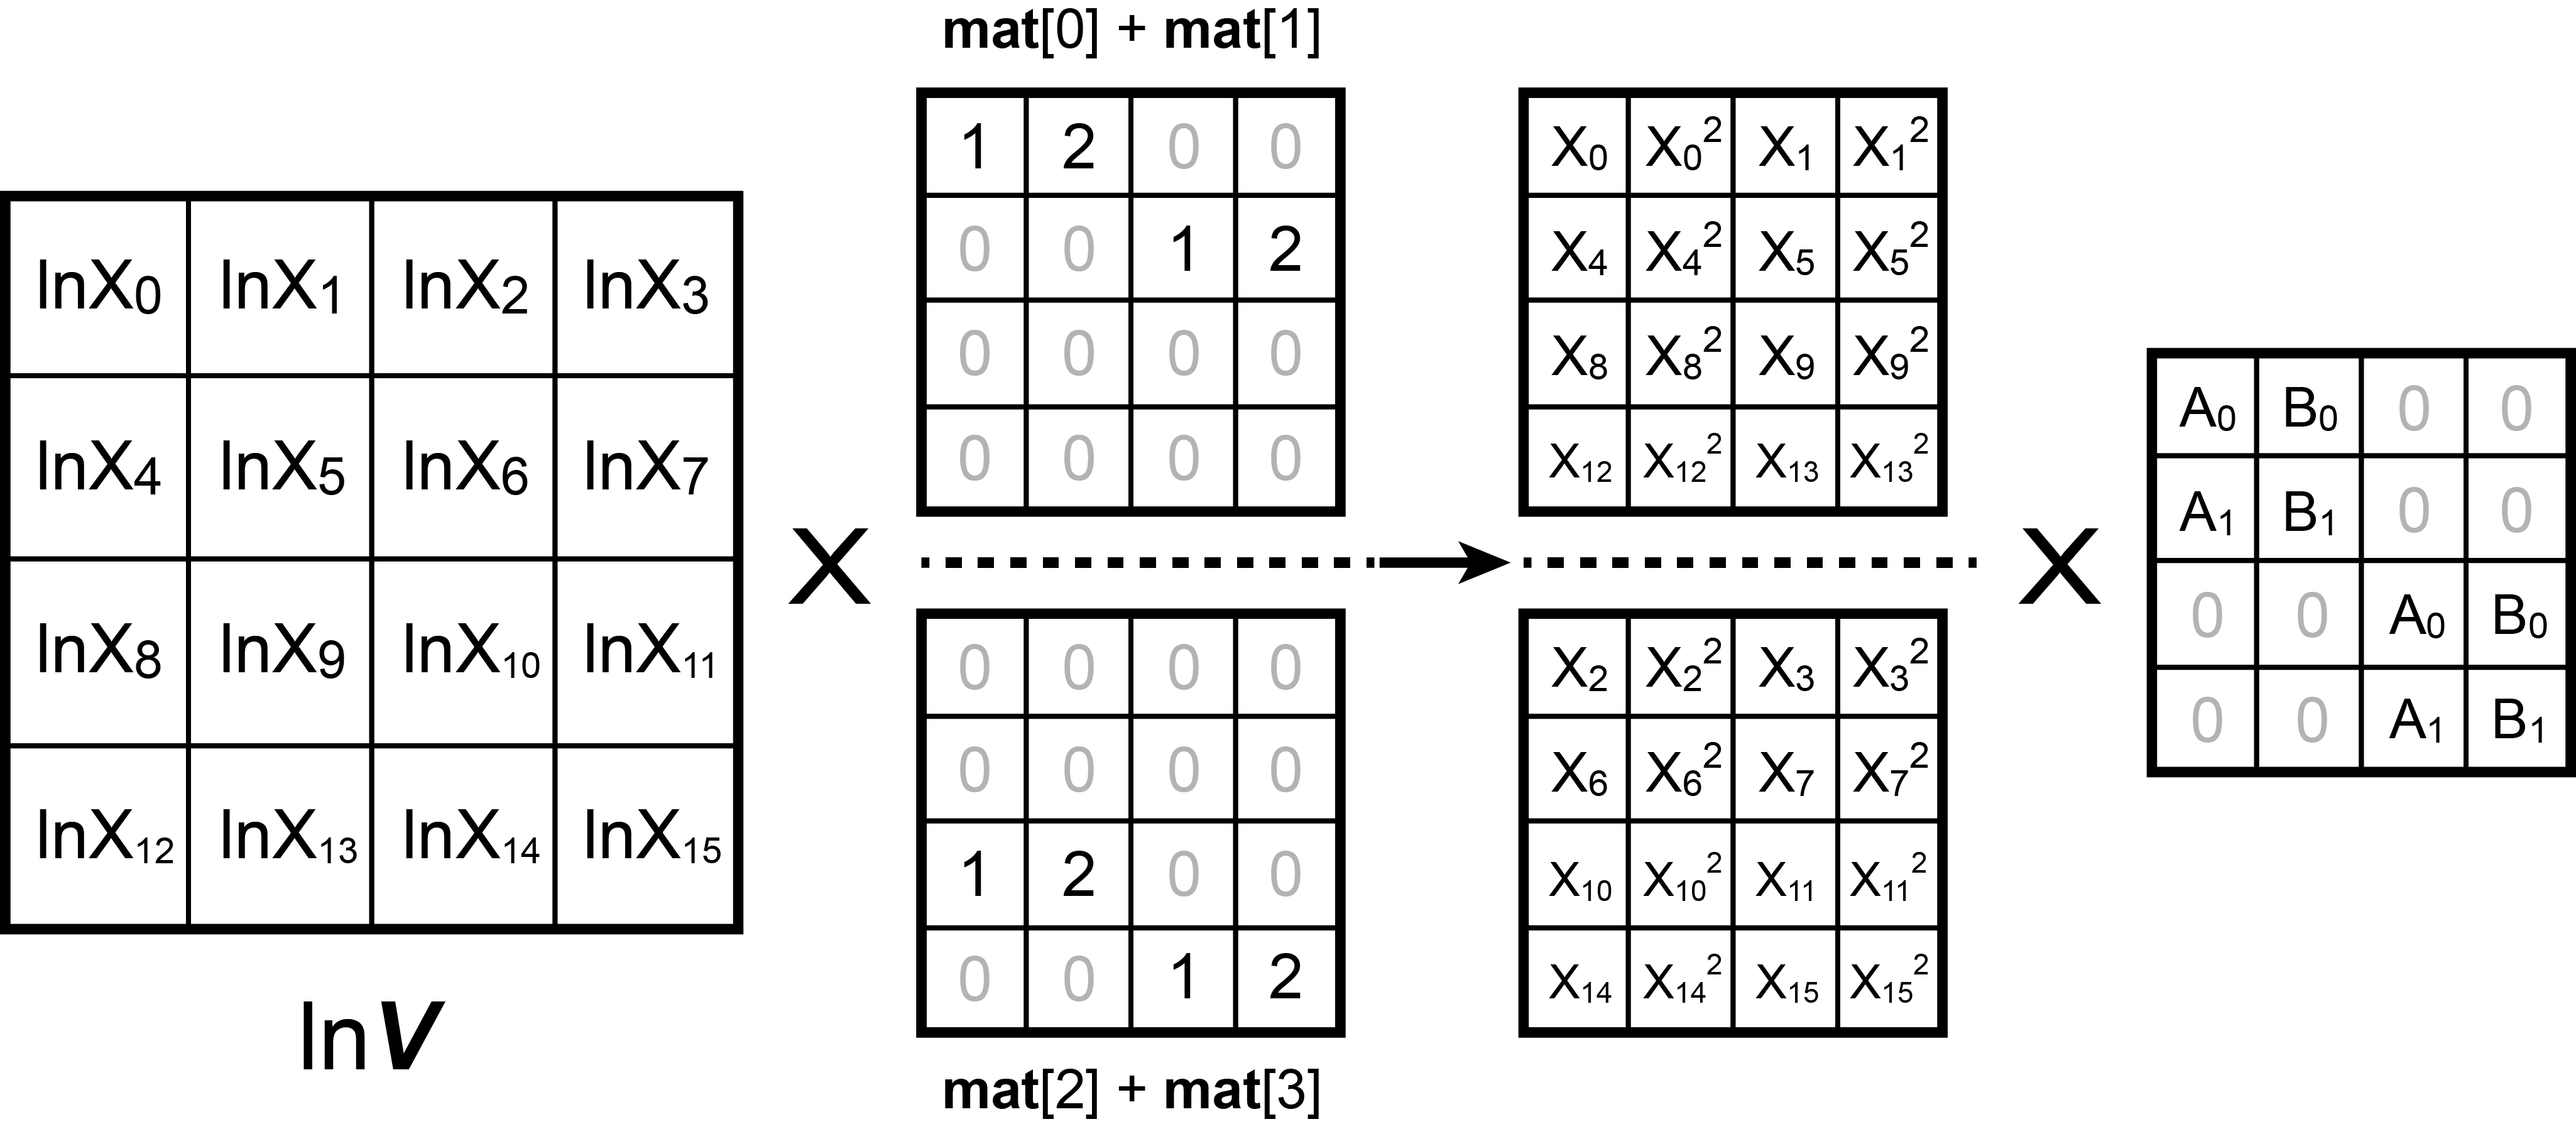
\includegraphics[scale=0.35]{figures/parallel.png}}
    \caption{Enhanced Cube-fx where $s = 4, k = 2, j = 2$}
    \label{fig:parallel}
    \end{figure}

To avoid the computation power waste, we propose an enhanced mapping for Cube-fx, which merges multiple matrices to the block diagonal matrices to reduce the number of Cube-fx loop steps. As shown in Fig. \ref{fig:parallel}, in the preparation stage, the Sequence Matrix $mat[0]$ and $mat[1]$ are merged into one single block-diagonal Sequence Matrix $mat[0] + mat[1]$, where the two non-zero columns of $mat[1]$ are moved to the third and fourth column of the $mat[0]$. Therefore, the result Variable Sequence matrix is a combination of the columns of the two related result matrices. Symmetrically, to fit the Variable Sequence matrix generated in the preparation stage, the block-diagonal Coefficient Matrix also combines the two original Coefficient Matrices but combines the rows of the matrices instead of the columns in the computation stage. As a result, all the elements of the result matrix are non-zero and valid, which means no computation power is wasted to compute zeros. Furthermore, the step number of the main loop is decreased to two, and the Matrix MAC Count is cut from eight to four, significantly reducing the execution time.

\begin{figure}[t]
    \centering{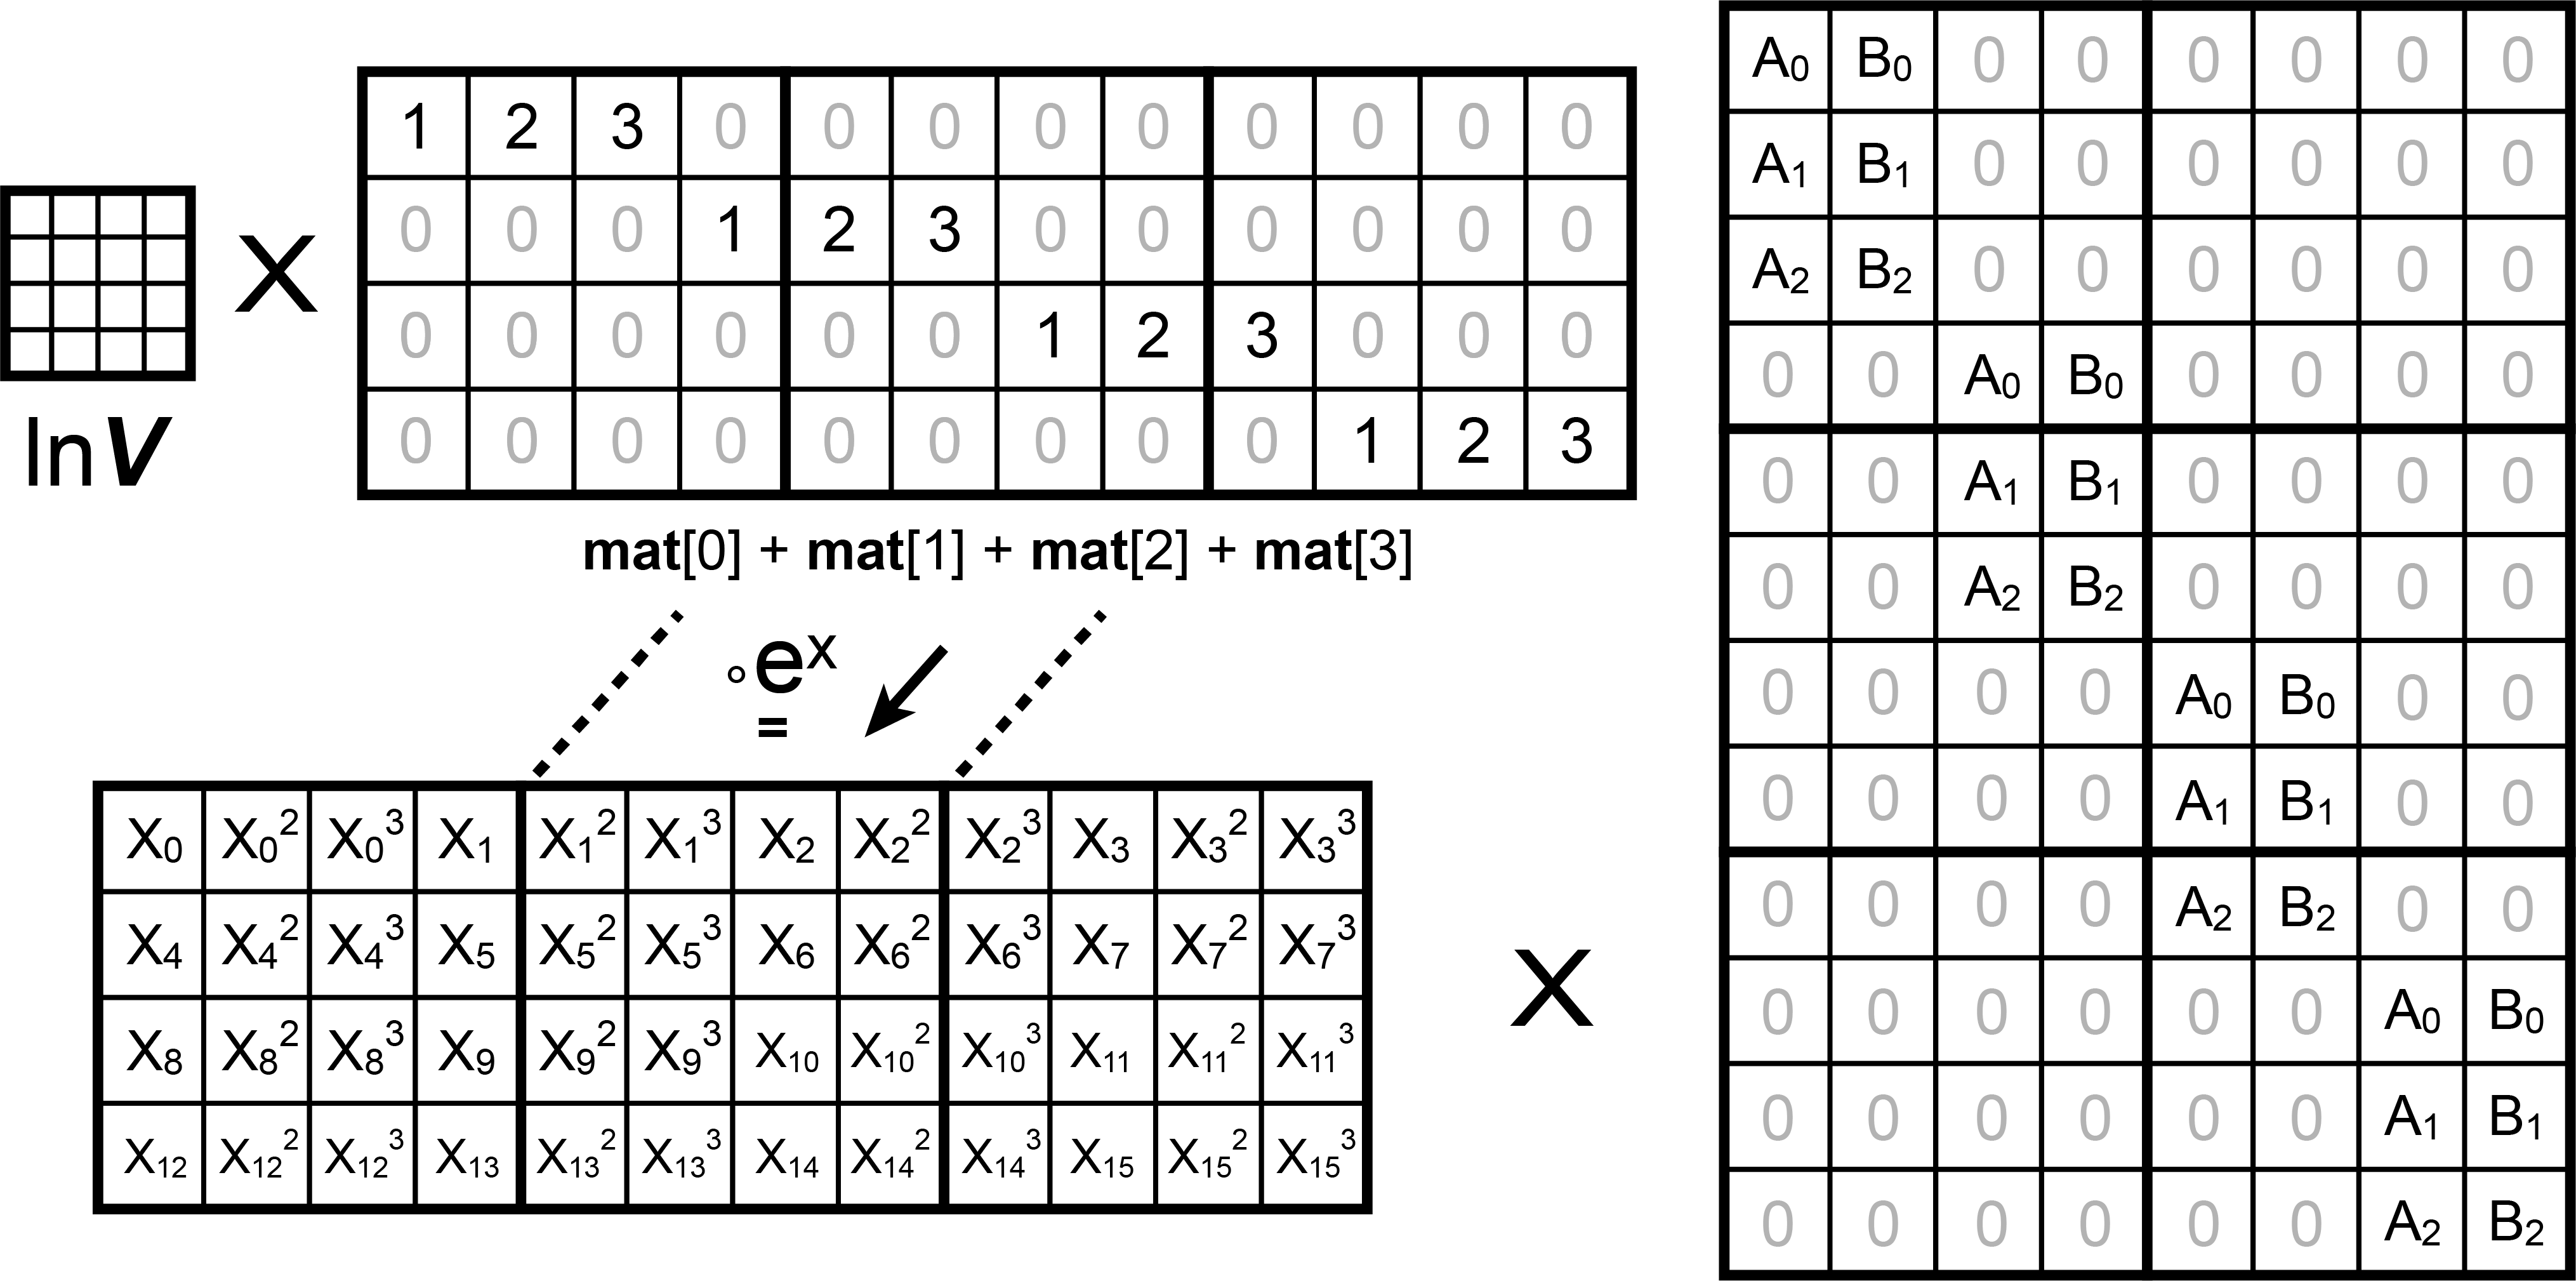
\includegraphics[scale=0.35]{figures/parallel_1.png}}
    \caption{Enhanced Cube-fx where $s = 4, k = 3, j = 2$}
    \label{fig:parallel_1}
    \end{figure}

However, the mapping cannot improve the efficiency of Cube-fx in all cases. As the example given in Fig. \ref{fig:parallel_1}, we increase the order number to three. Then, in the preparation stage, one Matrix MAC, whose side length is four, cannot simultaneously contain six non-zero columns of two Sequence Matrices. Therefore, to fully utilize the computation power, we can only fuse four original Sequence Matrices into three basic units of the Matrix MACs, whose total column number is 12. Since the matrices of a matrix multiplication should share the same $k$-dimension, the Coefficients Matrix must combine six matrices in the computation stage, whose row number is 12. The Matrix MAC Count of the enhanced Cube-fx increases to $(3 + 3 \times 2 = 9)$ compared to $(4 + 4 = 8)$ with naive Cube-fx. Hence, in this case, the enhanced Cube-fx mapping does not decrease the Matrix MAC Count but increases a lot instead. Therefore, in the following subsection, we analyze and quantify when Cube-fx needs further mapping and how to decide the number of merged Sequence Matrices.

\subsection{Quantification \label{sec:qua}}

For a Matrix MAC of the shape $(s \times s)$, let us consider an application of Cube-fx, where the Taylor polynomial order number is $k$, the evaluated function number is $j$, and the input data length is $(s \times s)$. 

\begin{figure}[t]
    \centering{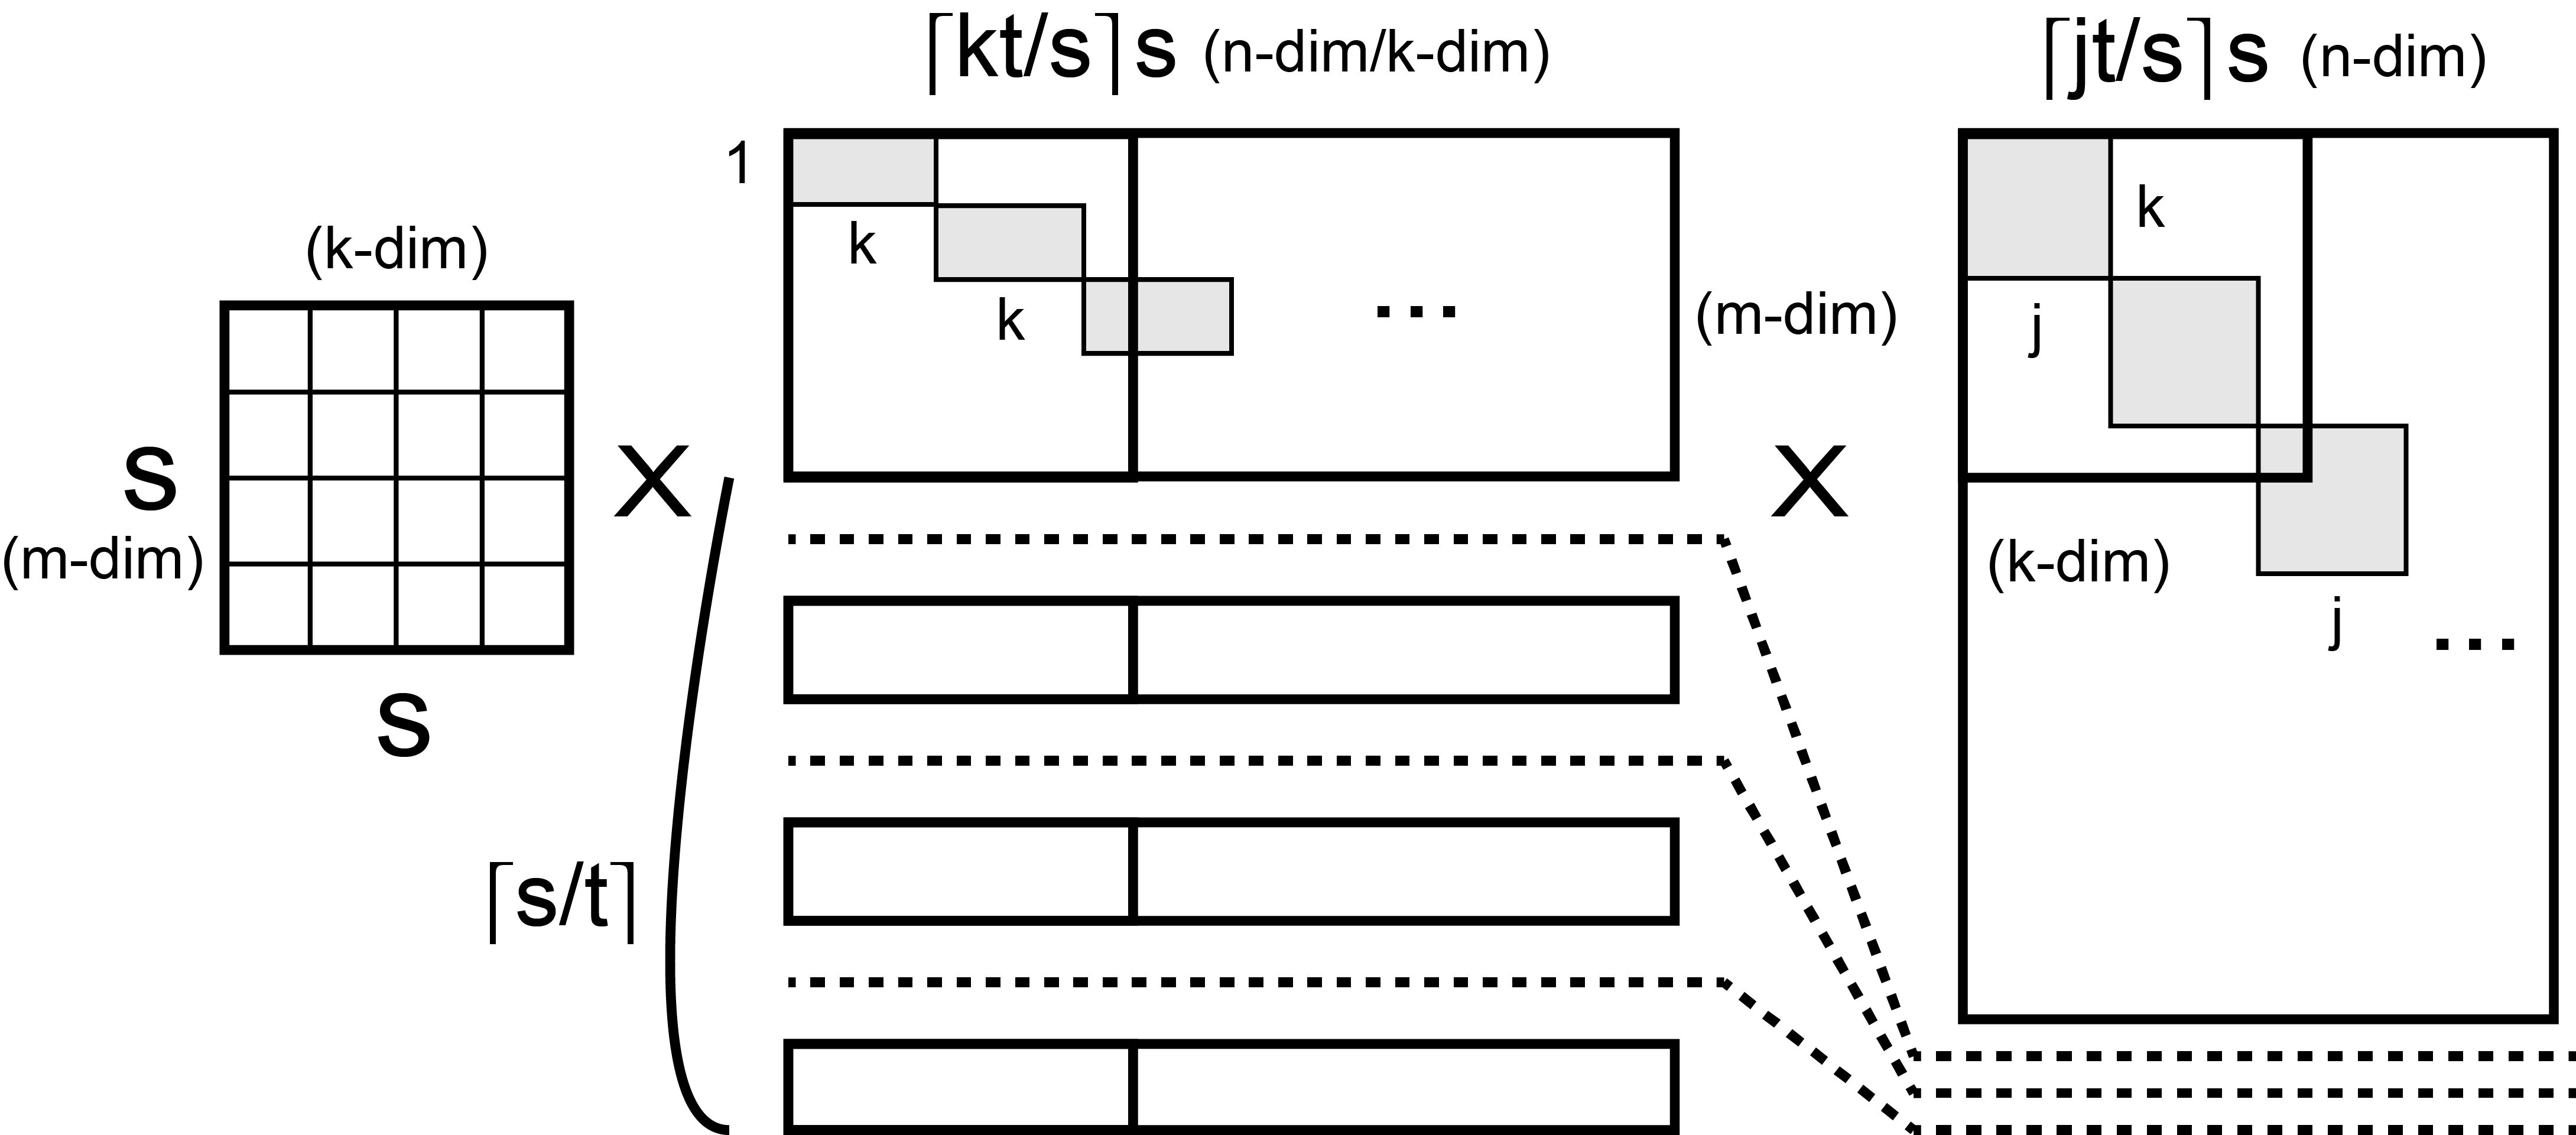
\includegraphics[scale=0.35]{figures/general.png}}
    \caption{Enhanced Cube-fx for General Cases}
    \label{fig:general}
    \end{figure}

In the preparation stage, since the order number is $k$, the shape of the non-zero data from each original Sequence Matrix is $(1 \times k)$. Let us merge $t$ original Sequence Matrices, as shown in Fig. \ref{fig:general}, where $t \in \mathbb{N}^{+}, 1 \le t \le s$. Then, the loop step $L$ of Cube-fx is:

\begin{equation}
    \label{eq:gen_1}
    \begin{aligned}
    L = \ceil*{\frac{s}{t}}
    \end{aligned}
    \end{equation}

% Then the $n$-dimension $D_{p_n}$ of the matrix multiplication is:

% \begin{equation}
%     \label{eq:gen_2}
%     \begin{aligned}
%     D_{p_n} = \ceil*{\frac{kt}{s}} \cdot s
%     \end{aligned}
%     \end{equation}

where $\ceil*{x}$ is the ceiling function. The Matrix MAC Count of the preparation stage $M_{p}$ for one loop step is:

\begin{equation}
    \label{eq:gen_3}
    \begin{aligned}
    M_{p} = \ceil*{\frac{kt}{s}} \cdot s \cdot \frac{s^2}{s^3} = \ceil*{\frac{kt}{s}}
    \end{aligned}
    \end{equation}

Similarly, in the computation stage, the Matrix MAC Count of the computation stage $M_c$ for one loop step is:

% the Coefficient Matrix is merged by $t$ original Coefficient Matrices. Therefore, the $n$-dimension $D_{C_n}$ of the matrix multiplication is:

% \begin{equation}
%     \label{eq:gen_4}
%     \begin{aligned}
%     D_{C_n} = \ceil*{\frac{jt}{s}} \cdot s
%     \end{aligned}
%     \end{equation}

% Since the $k$-dimension of the matrix multiplication equals the $n$-dimension in the preparation stage's matrix multiplication, 

\begin{equation}
    \label{eq:gen_5}
    \begin{aligned}
    M_c = \ceil*{\frac{jt}{s}} \cdot \ceil*{\frac{kt}{s}} \cdot s^2 \cdot \frac{s}{s^3} = \ceil*{\frac{jt}{s}} \cdot \ceil*{\frac{kt}{s}}
    \end{aligned}
    \end{equation}

Hence, the Matrix MAC Count for $L$ steps $M$ is:

\begin{equation}
    \label{eq:gen_6}
    \begin{aligned}
    M = L \cdot (M_p + M_c)
      = \ceil*{\frac{s}{t}} \cdot \ceil*{\frac{kt}{s}} \cdot (1 + \ceil*{\frac{jt}{s}})
    \end{aligned}
    \end{equation}

In addition, the size of the three matrices in Cube-Fx transferred from the global memory is formulated as:

\begin{equation}
    \label{eq:gen_7}
    \begin{aligned}
    S_{z} &= s^2 + \ceil*{\frac{s}{t}} \cdot (s^2 \cdot \ceil*{\frac{kt}{s}} + s^2 \cdot \ceil*{\frac{kt}{s}} \cdot \ceil*{\frac{jt}{s}}) \\
          &= s^2 + \ceil*{\frac{s}{t}} \cdot \ceil*{\frac{kt}{s}} \cdot s^2 \cdot (1 + \ceil*{\frac{jt}{s}})
    \end{aligned}
    \end{equation}

% \begin{equation}
%     \label{eq:gen_7}
%     \begin{aligned}
%     S_{z} = s^2 + \ceil*{\frac{s}{t}} \cdot \ceil*{\frac{kt}{s}} \cdot s^2 \cdot (1 + \ceil*{\frac{jt}{s}})
%     \end{aligned}
%     \end{equation}

We formulate an integer programming (IP) problem:

\begin{equation}
    \label{eq:optimized_3}
    \begin{aligned}
        min&\quad M + b S_{z} = \ceil*{\frac{s}{t}} \cdot \ceil*{\frac{kt}{s}} \cdot (1 + \ceil*{\frac{jt}{s}}) \cdot (1+ bs ^ 2) + bs ^ 2 \\
        s.t.& \quad t \in \mathbb{N}^{+}, 1 \le t \le s
    \end{aligned}
\end{equation}

where $b$ is a constant value combining the Matrix MAC Count with the data movement. Since the data movement size is proportional to the Matrix MAC Count, the actual value of $b$ is trivial in the optimization problem. Intuitively, increasing $t$ can decrease the loop step $L$ but raise the $n$-dimention in both the preparation and computation stages. 

\section{Evaluation \label{sec:5}}

In this section, we evaluate the precision and efficiency performance of Cube-fx on Huawei Ascend 310 and Ascend 910B AI processors. All the experiments given in the evaluation are programmed as Ascend kernels (similar to CUDA Kernels) with Tensor Iterator Kernel (TIK, a Python library) based on a Huawei full-stack programming framework called AI heterogeneous Compute Architecture (CANN). Since Cube-fx can naturally execute in parallel, we only activate a single core during the evaluation for simplicity. Therefore, for Ascend 310 processors, we activate one Cube Unit with one Vector Unit; for Ascend 910B processors, we activate one Cube Unit with two Vector Units (one Cube Core with two Vector Cores), the most elementary structure. All the experiment results are evaluated from Huawei's official profiler tool, \textit{msprof}, which reports the detailed runtime information of a DaVinci Kernel. The data type we used during the evaluation is FP16, one of AI applications' most popular data types.

\subsection{Computation Precision Evaluation \label{Sec: 4.1}}

\begin{table}[tb]
  \label{tab:precison}
  \caption{Precision Evaluation for Float16}
  \begin{center}
  
  \scalebox{0.75}{
      \begin{tabular}{c|c|c|c|c|c|c|c}
      \toprule[1pt]
          \textbf{Function} &
          \textbf{Input} &
          \textbf{Numpy} &
          \makecell[c]{\textbf{COR-} \\ \textbf{DIC}} &
          \makecell[c]{\textbf{Horner's} \\ \textbf{Order 8}} &
          \makecell[c]{\textbf{Cube-fx} \\ \textbf{Order 8}} &
          \makecell[c]{\textbf{Horner's} \\ \textbf{Order 16}} &
          \makecell[c]{\textbf{Cube-fx} \\ \textbf{Order 16}} \\
      \midrule[0.5pt]

      \multirow{3}*{\makecell[c]{sin(x)}} 
      ~ & 0.14 & 0.1395 & 0.0\% & 0.012\% & 0.012\% & 0.012\% & 0.012\% \\
      ~ & 0.52 & 0.4969 & 0.0\% & 0.011\% & 0.011\% & 0.011\% & 0.011\% \\
      ~ & 2.08 & 0.8731 & 0.0\% & 0.178\% & 0.178\% & 0.046\% & 0.046\% \\
      \midrule[0.5pt]

      \multirow{3}*{\makecell[c]{cos(x)}}
      ~ & 0.14 & 0.9902 & 0.0\% & 0.002\% & 0.002\% & 0.002\% & 0.002\% \\
      ~ & 0.52 & 0.8678 & 0.0\% & 0.017\% & 0.017\% & 0.017\% & 0.017\% \\
      ~ & 2.08 & -0.4875 & 0.0\% & 1.917\% & 1.917\% & 0.214\% & 0.214\% \\
      \midrule[0.5pt]

      \multirow{3}*{\makecell[c]{tan(x)}}
      ~ & 0.14 & 0.1409 & 0.0\% & 0.049\% & 0.049\% & 0.049\% & 0.049\% \\
      ~ & 0.52 & 0.5726 & 0.0\% & 0.052\% & 0.052\% & 0.034\% & 0.034\% \\
      ~ & 2.08 & -1.791 & 0.0\% & 1181\% & 1180\% & 11160\% & 11160\% \\
      \midrule[0.5pt]

      \multirow{3}*{\makecell[c]{tanh(x)}}
      ~ & 0.14 & 0.1391 & 0.0\% & 0.049\% & 0.049\% & 0.049\% & 0.049\% \\
      ~ & 0.52 & 0.4777 & 0.0\% & 0.017\% & 0.017\% & 0.017\% & 0.017\% \\
      ~ & 2.08 & 0.9693 & 0.0\% & 597.3\% & 595.3\% & 5649\% & 5620\% \\
      \midrule[0.5pt]

      \multirow{3}*{\makecell[c]{Sig- \\ moid(x)}}
      ~ & 0.14 & 0.5349 & 0.0\% & 0.040\% & 0.040\% & 0.040\% & 0.040\% \\
      ~ & 0.52 & 0.6271 & 0.0\% & 0.031\% & 0.031\% & 0.031\% & 0.031\% \\
      ~ & 2.08 & 0.8889 & 0.0\% & 1.239\% & 1.184\% & 0.134\% & 0.134\% \\
      \midrule[0.5pt]

      \multirow{3}*{\makecell[c]{GELU(x)}}
      ~ & 0.14 & 0.0778 & - & 0.034\% & 0.034\% & 0.049\% & 0.049\% \\
      ~ & 0.52 & 0.3632 & - & 0.021\% & 0.021\% & 0.021\% & 0.021\% \\
      ~ & 2.08 & 2.0410 & - & 14.17\% & 14.17\% & 0.289\% & 0.194\% \\
      \bottomrule[1pt]

      \end{tabular}
  }
  \end{center}
\end{table}

We first evaluate the computation precision of the Cube-fx. We use six sample functions with three different inputs, including trigonometric functions and activation functions in neural networks, to compare the precision of Cube-fx with CORDIC and Horner’s Method, respectively. CORDIC (COordinate Rotation DIgital Computer) \cite{DBLP:journals/tc/Volder59} is an iterative algorithm used to efficiently calculate trigonometric, hyperbolic, exponential, and logarithmic functions. The core idea of CORDIC is to represent calculations as a sequence of vector rotations in a plane, where each rotation is chosen to progressively bring the resulting vector closer to the desired angle. This iterative process avoids the need for multiplications, making it particularly well-suited for hardware implementations where computational efficiency is critical. The two algorithms based on Taylor polynomials are expanded around $x = 0$. The error rates are calculated as the percentage difference between the output of the algorithm and the output of Numpy, a Python library for scientific computing.

First, CORDIC reports $0.000\%$ error rates with the iteration of 8, which shows extremely high precision. The reason is that CORDIC is accurate to the bit of its iteration number, which is even higher than the precision of FP16. While the CORDIC implementations of $tanh(x)$ and $Sigmoid(x)$ are proposed by former researchers \cite{DBLP:conf/iscas/ChenJLLFLY20}, CORDIC for $GELU(x)$ is still absent, which we do not list in the table. The other two algorithms based on Taylor polynomials, including Cube-fx, report a few higher error rates. Generally, except for the outliers, the average error rates of Cube-fx are $1.112\%$ and $0.058\%$ for the order numbers 8 and 16, respectively. For comparison, the average error rates of Horner's Method are $1.115\%$ and $0.063\%$ for the order numbers 8 and 16. As for $tan(x)$ and $tanh(x)$ with the input $2.08$, the high error rates are caused by the fact that $2.08$ is out of the radius of convergence $(-\frac{\pi}{2}, \frac{\pi}{2})$ and diverges.

The evaluation results indicate that Cube-fx has comparable or lower error rates than Horner's method for most cases. Although the precision of Cube-fx is much lower than CORDIC, the errors are caused by the theoretical limit of Taylor expansion but not Cube-fx itself. In other words, compared to the pure multiplications and additions of Horner's method, the logarithm and exponent operations of Cube-fx do not bring extra errors to the computation and even reduce the errors for some cases. Therefore, for applications where Taylor expansion has met the precision requirements, Cube-fx would be safe to replace other implementations, including Horner's Method.

\subsection{Full Matrix MAC Evaluation \label{Sec: 4.2}}

In this subsection, we compare the execution time of Cube-fx with the naive Taylor expansion, CORDIC, Horner's Method, Estrin's Scheme, and Motzkin's Method. The naive Taylor implementation is used in SymPy \cite{10.7717/peerj-cs.103} for its \verb|series()| function, which builds the variable sequences and performs the multiplications with the Taylor polynomial coefficients. All implementations are SIMD-optimized using vectorized operations. For Taylor-based algorithms, we use an order of 16, matching the side length of the Matrix MACs $(k = s = 16)$ to utilize the Matrix MACs on Ascend processors fully. For CORDIC, we use 4 iterations, providing high precision as discussed in Sec. \ref{Sec: 4.1}. To ensure a fair comparison, all functions evaluated are trigonometric, avoiding the need for extra pre- and post-processing for CORDIC. We analyze the kernel execution time for varying numbers of evaluated functions, using input data sizes of 16384 and 32768 on Ascend 310 processors, and 1638400 and 3276800 on Ascend 910B processors, which represent the length of the input data sequence being processed.

\begin{figure}[thp]
    \centering{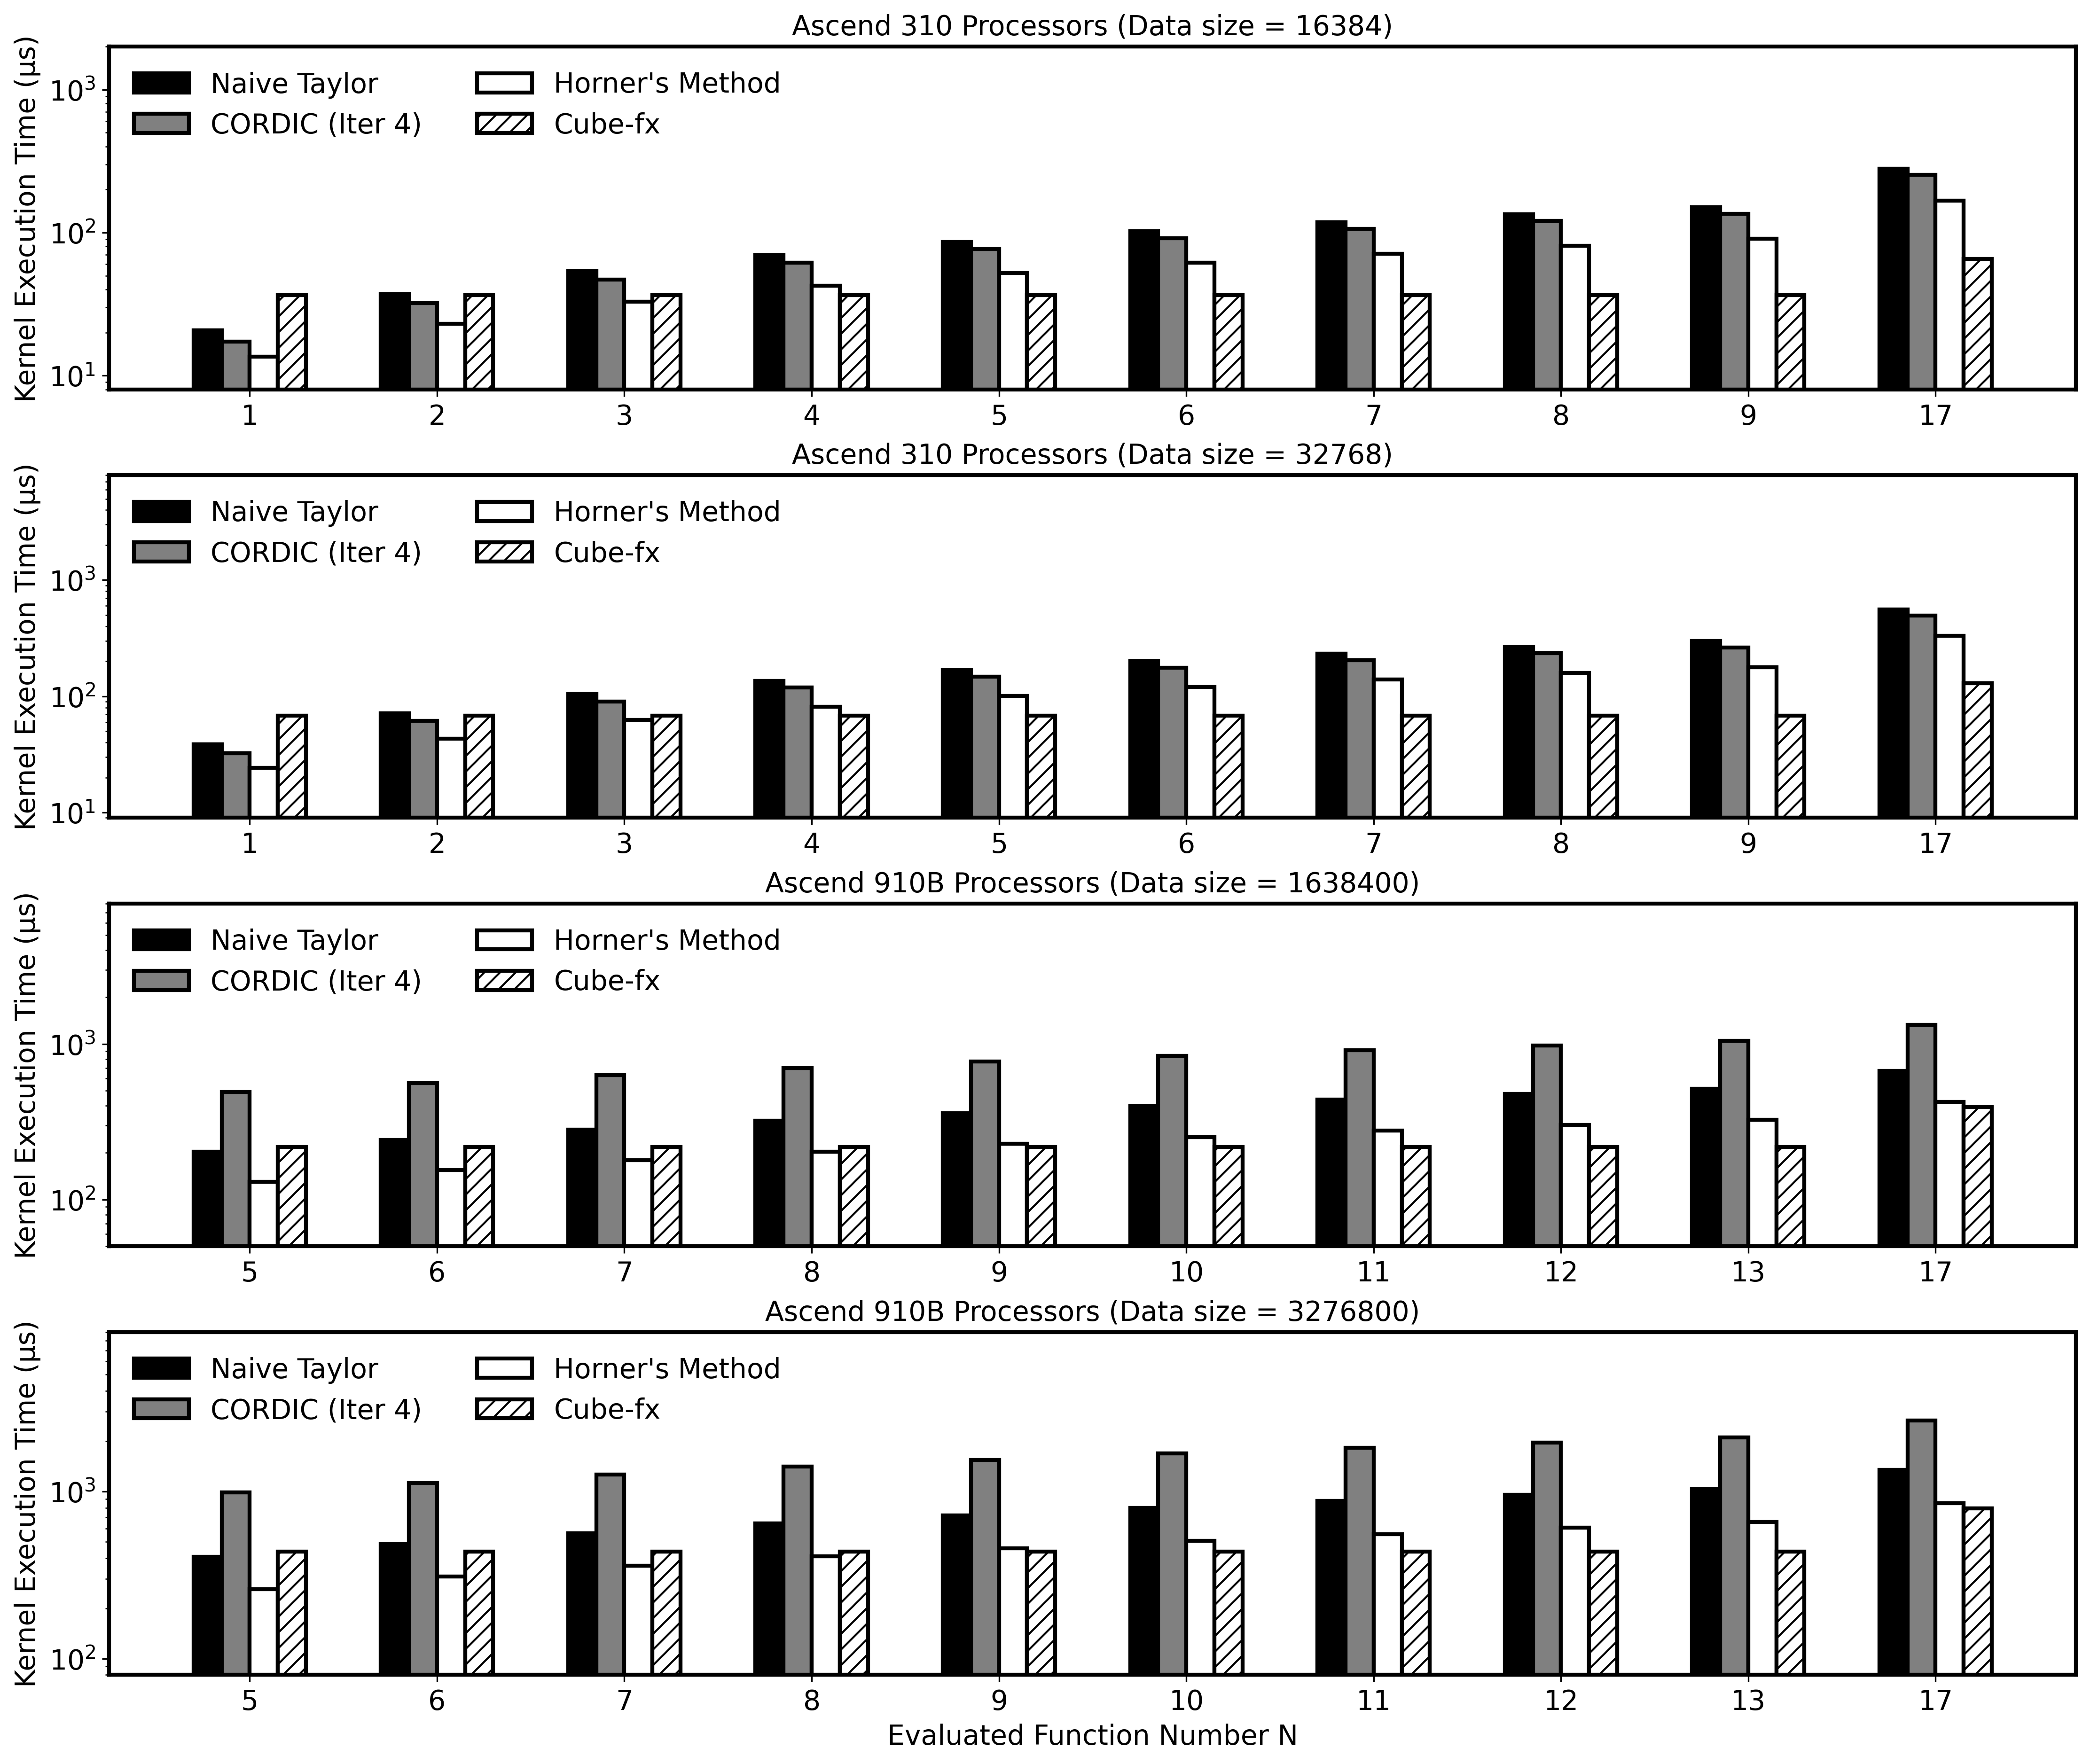
\includegraphics[scale=0.5]{figures/compare.png}}
    \caption{The execution time evaluations (order number = 16)}
    \label{fig:compare}
    \end{figure}

\subsubsection{Results}

Fig. \ref{fig:compare} illustrates the evaluation results. Generally, all the algorithms grow with the increment of the evaluated function number. Since all the algorithms traverse the data for execution, the execution time linearly increases with the data sizes. Cube-fx shows significant speedups compared to other implementations when the number of the evaluated functions is large enough. For the results on Ascend 310 processors, Cube-fx shows an average result of $2.73\times$ speedup compared to the naive Taylor expansion implementation, $6.06\times$ speedup compared to CORDIC, $1.64\times$ speedup compared to Horner's Method, $1.53\times$ speedup compared to Estrin's Scheme and $1.85\times$ speedup compared to Motzkin's Method. For the results on Ascend 910B processors, Cube-fx reports $1.63\times$ speedup compared to the naive Taylor expansion implementation, $3.52\times$ speedup compared to CORDIC, $1.28\times$ speedup compared to Horner's Method, $1.20\times$ speedup compared to Estrin's Scheme and $1.42\times$ speedup compared to Motzkin's Method. 

When the evaluation function number is $1$, Horner's Method is $2.68\times$ and $6.02\times$ faster than Cube-fx, Estrin's Scheme is $2.87\times$ and $6.38\times$ faster, and Motzkin's Method reaches $2.38\times$ and $4.76\times$ on Ascend 310 and 910B processors, respectively. However, when the number is $9$, Cube-fx reversely reports $2.48\times$ and $1.05\times$, $2.48\times$ and $1.19\times$, and $2.80\times$ and $1.42\times$ speedup instead. In detail, as shown in Fig. \ref{fig:compare}, on Ascend 310 processors, when the evaluation function number is larger than 3, Cube-fx reports better efficiency than other implementations and keeps enlarging the performance. On Ascend 910B processors, the turning point is 8. The main reason for the results is that compared to the time complexity we discussed in Sec. \ref{sec:3} for Cube-fx, the time complexity of general Cube-fx is $O(Nk + \ceil{N / s} \ceil{k / s} + \ceil{N / s} \ceil{k / s} \ceil{j / s})$, where the execution time of Cube-fx increases every $s$ evaluated functions. The ceiling functions are added here because the Matrix MAC must complete a basic unit $(s \times s \times s)$ of matrix multiplication each time, as mentioned in Sec. \ref{sec:qua}. Therefore, for the number of evaluated functions within $[1, 16]$, Cube-fx reports a nearly constant execution time, while the other implementations increase linearly. As for the evaluated function number of 17, where $\ceil{17 / 16} = 2$, the execution time of Cube-fx finally increases to $1.79\times$ of the previous results on Ascend 310 processors. On Ascend 910B processors, the execution time of Cube-fx with the evaluated function number 17 increases to $1.81\times$. In addition, by activating the Matrix MACs, we reduce the utilization rate of the weak Vector Units to $56.38\%$ on Ascend 310 and $34.95\%$ on Ascend 910B, which move most of the workloads to the Matrix MACs.

\subsubsection{Discussion \label{sec:dis_1}}

The results above reveal that Cube-fx performs much better on Ascend 310 processors than on Ascend 910B processors. Based on the hardware structure, this subsection discusses the reasons and the potential improvements.

\begin{figure}[tbp]
  \centering{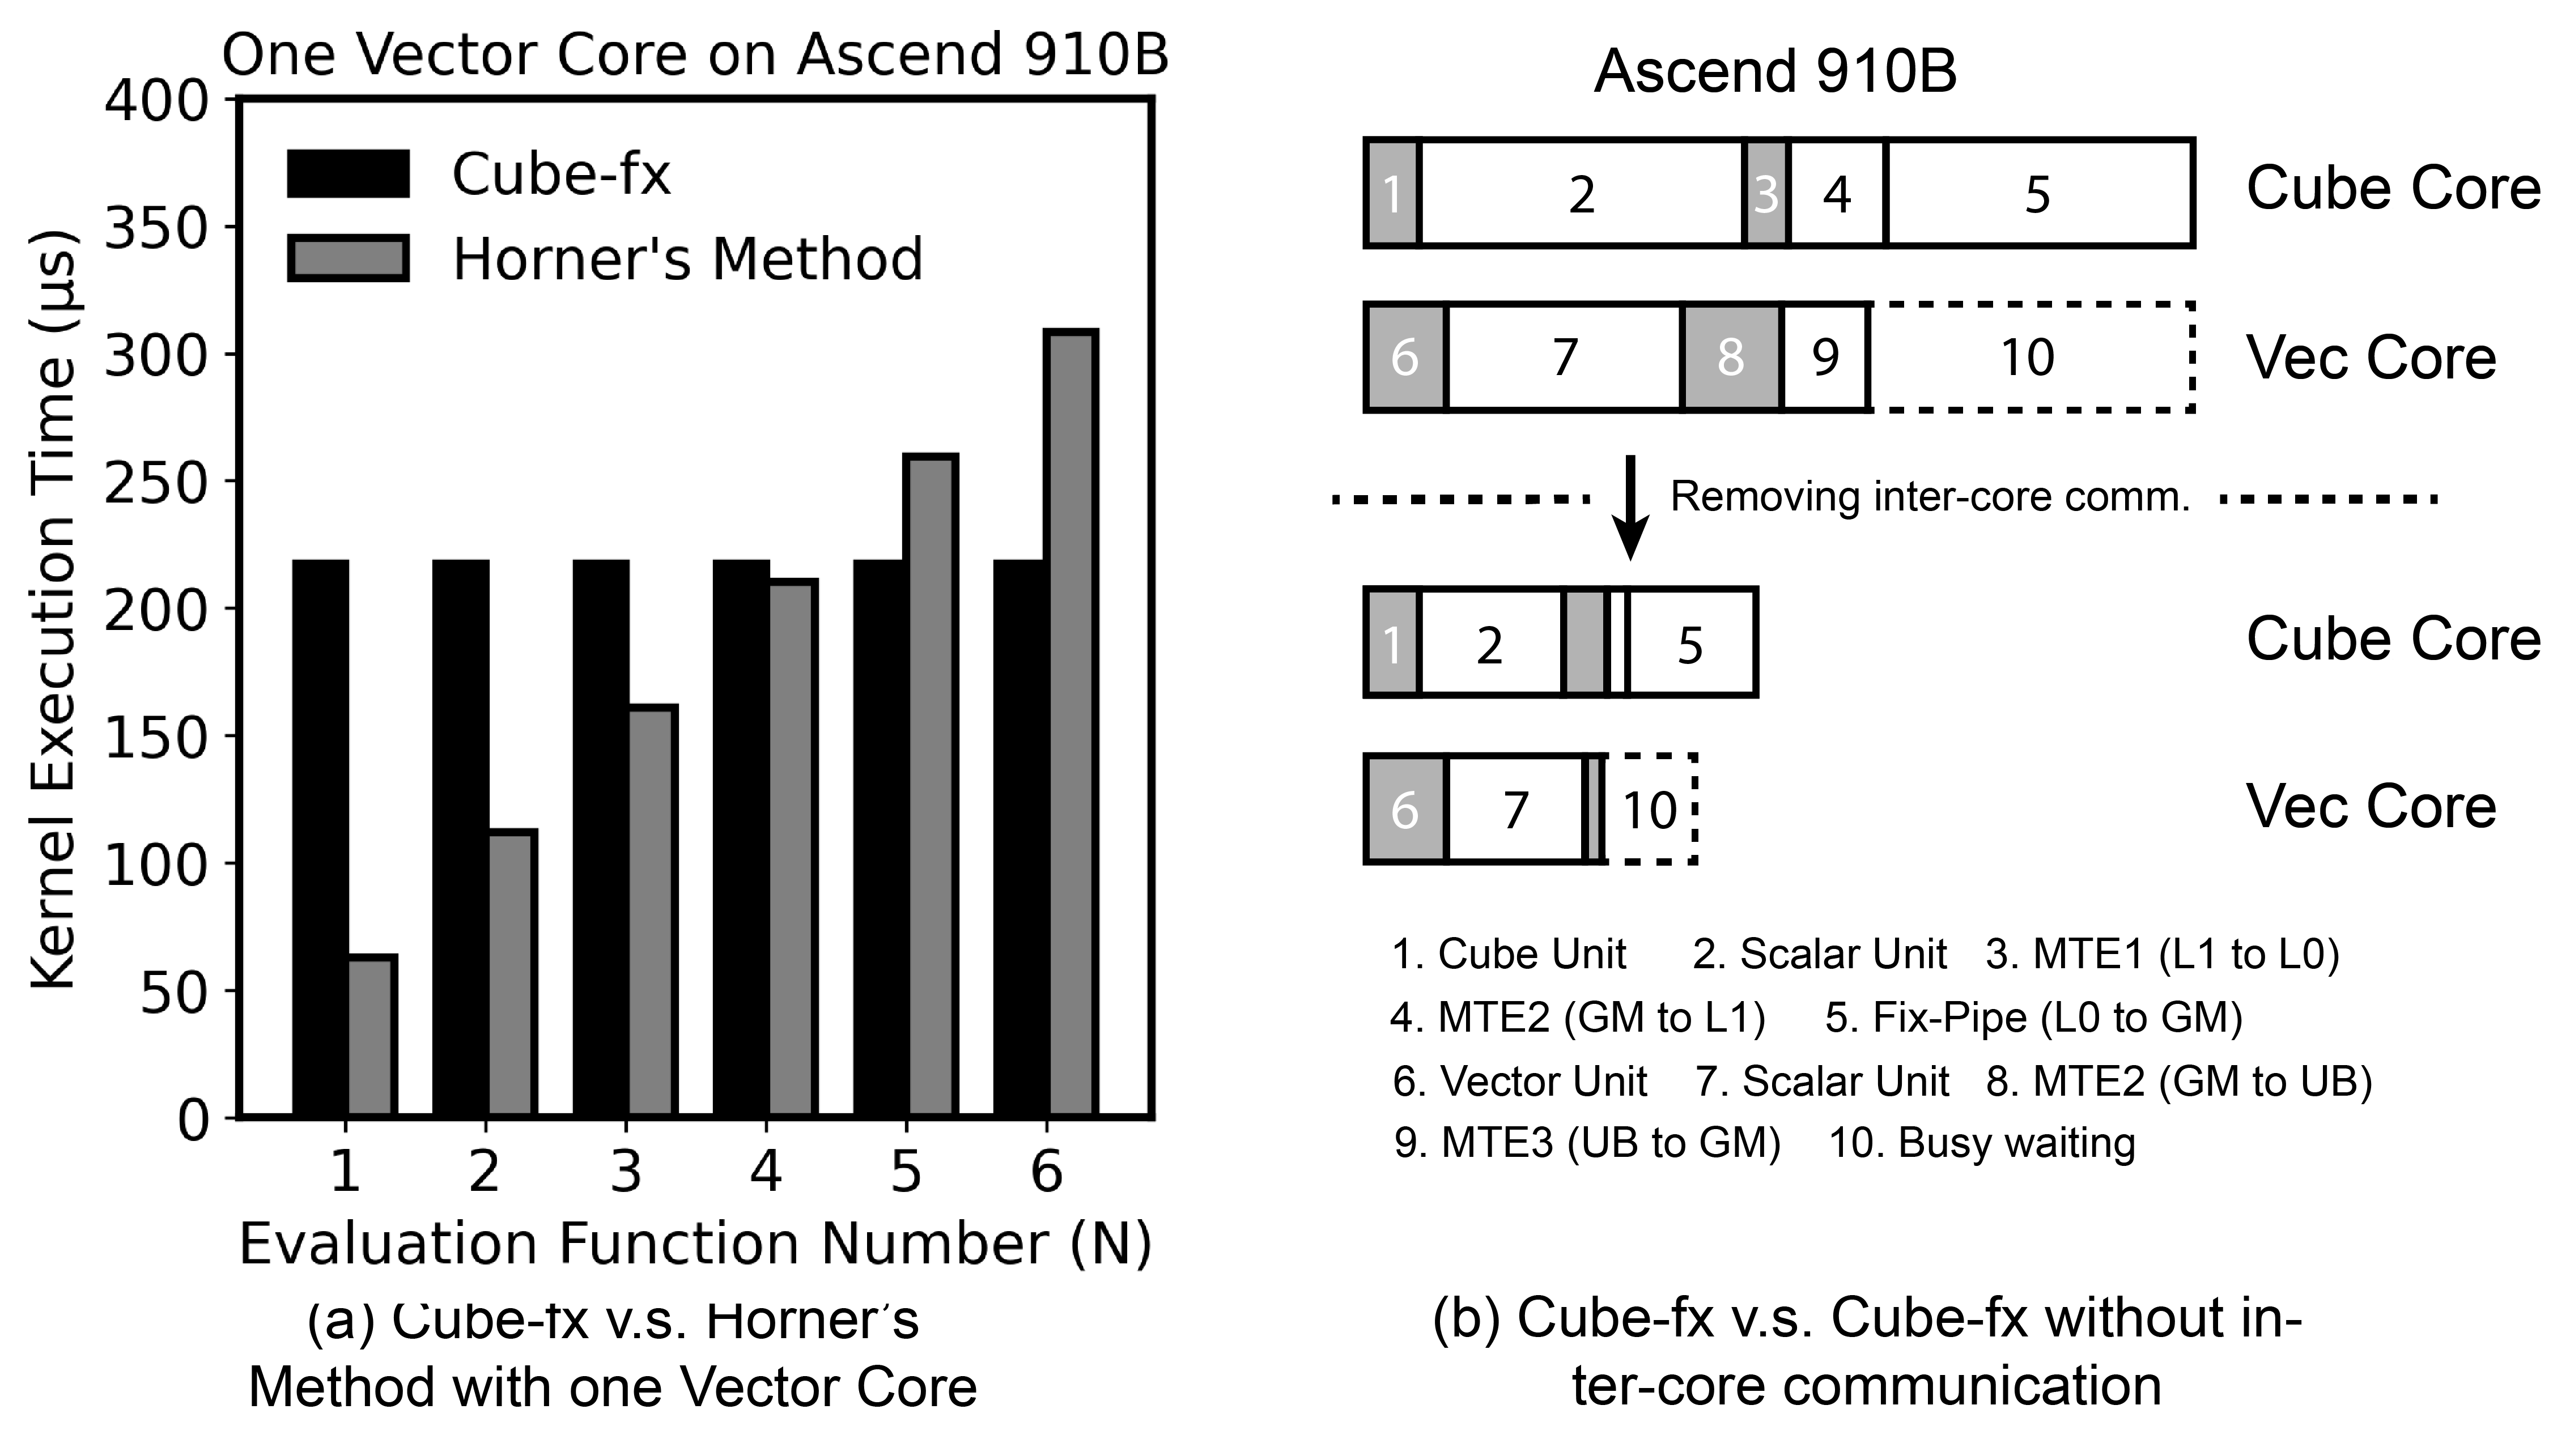
\includegraphics[scale=0.35]{figures/discussion.png}}
  \caption{Performance comparison of modified implementations on Ascend 910B}
  \label{fig:disc}
  \end{figure}

First, the most significant reason is that Ascend 910B processors have two Vector Units, which provide double vectorized computation power compared to Ascend 310 processors. As discussed in Sec. \ref{sec_1_2_2}, the Cube Unit of Ascend 310 processors is more dominant than Ascend 910B, which empowers our Cube-fx more than other implementations. When we disable one Vector Unit of Ascend 910B processors, Cube-fx reports similar accelerations compared with Horner's Method on Ascend 310 processors. When the evaluated function number is 4, Cube-fx performs only $1.03\times$ of execution time compared with Horner's Method, as shown in Fig. \ref{fig:disc}(a). Since Cube-fx only contains a small part to be executed on Vector Units, the increment of the Vector Units cannot improve to the majority of the algorithm. The performance of Cube-fx is much more sensitive to the number of the Cube Units, as it highly utilizes the units. Therefore, Cube-fx performs better on Ascend 310 processors, the edge-computing hardware without rich vectorized computation resources.

Second, since Cube-fx heavily relies on the cooperation of the two computation units, the data communication between Cube Core and Vector Core heavily influences the performance of Cube-fx. As shown in Fig. \ref{fig:dav}, to transfer data between the Cube Units and Vector Units, Ascend 910B processors must write the results back to the global memory and then read from it. The IO operations contribute to most of the execution time compared with the execution on Ascend 310 processors. Fig. \ref{fig:disc}(b) shows the results of removing the data communication between Cube Core and Vector Core by manually deleting the related instructions. We illustrate the execution of Cube Core and Vector Core separately in Fig. \ref{fig:disc}(b). Each bar refers to the execution time of each hardware unit on the according core. As a result, the modified version without data communication (lower subgraph) reports a $43.46\%$ reduction in the execution time compared with the original version (upper subgraph). Notice that in addition to the reduction of Fix-Pipe and MTE3 Units, the execution time of the Scalar Unit also reduces, which computes the memory address of the data communication. Furthermore, the busy waiting time of Vector Core is significantly reduced to $28.55\%$ of that in the original Cube-fx. The busy waiting time comprises the idleness and inter-core synchronization we discussed in Sec. \ref{sec:3.3}. Even though we optimize the algorithm for potential concurrent execution, the extra inter-core data communication severely extends the execution periods on both units, which the concurrent execution cannot overlap and hide.

\subsubsection{AI Cube + AI Vector vs AI Cube + CPU Vector}

Since previous experiments identified vector units as a potential bottleneck, this subsection investigates the performance of integrating CPU vector units with Ascend Cube Units. We evaluate the performance of Cube-fx by combining CPU Vector Units (Arm Neon \cite{neon}) with Ascend Cube Units and compare it against using only Ascend processors. The input data sizes are configured as 16384 for Ascend 310 and 1638400 for Ascend 910B processors. In contrast to the previous experiments, where the Huawei profiler, \textit{msprof}, was used for performance measurement, we use an end-to-end wall clock approach here. This change is because of the limitation that the profiler cannot be used to measure execution times on the IO and CPU sides.
  
\begin{figure}[tbp]
    \centering{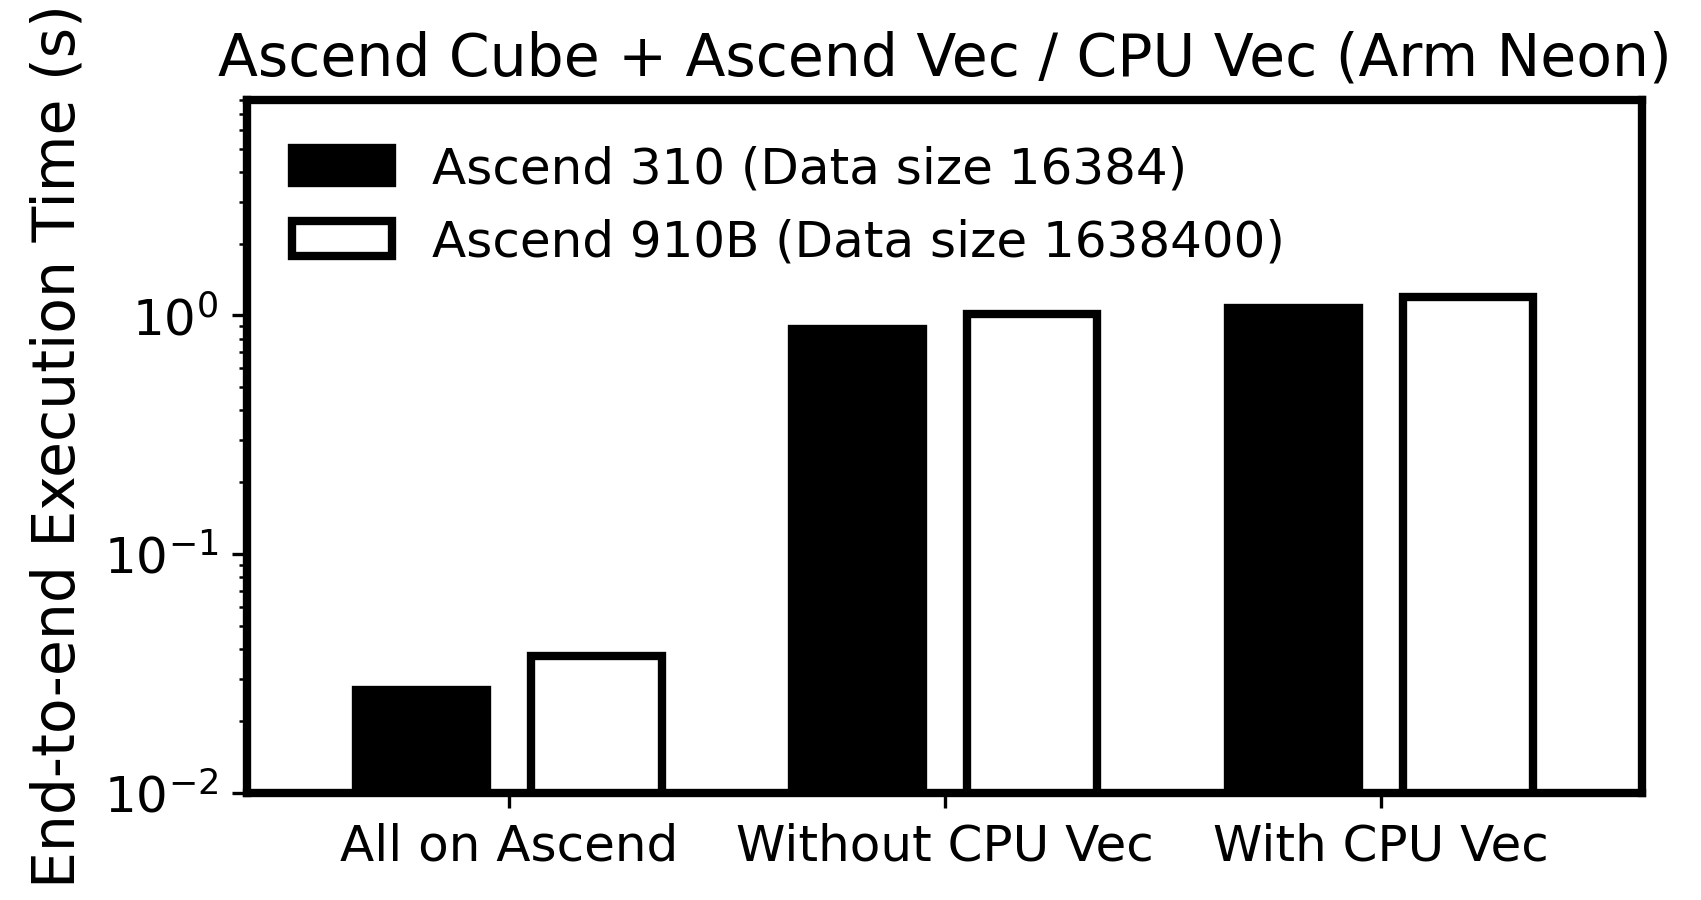
\includegraphics[scale=0.58]{figures/cpu_ai.png}}
    \caption{The comparison between (AI Cube + AI Vector) and (AI Cube + CPU Vector)}
    \label{fig:cpu_ai}
    \end{figure}
  
As shown in Fig. \ref{fig:cpu_ai}, performing all the computations on the AI processors leads to much faster execution compared to using CPUs for vectorized computations, achieving speedups of $39.81\times$ and $31.67\times$ on Ascend 310 and 910B processors, respectively. We also included a scenario without using the CPUs for vectorized computations, labeled as 'Without CPU Vec' in Fig. \ref{fig:cpu_ai}. These results indicate that the execution time was still $32.63\times$ and $26.89\times$ longer compared to using only the AI processors. The main reason for this is that transferring data between the AI processors and CPUs takes too much time. Additionally, doing vectorized computations on the CPU is inherently slower. Firstly, Arm Neon Instructions do not directly support exponentiation or logarithmic functions, requiring extra processing and evaluation. Secondly, the CPU SIMD units (Huawei Kunpeng) are much narrower compared to Ascend Vector Units (8 float16 \cite{kunpeng} vs 128 float16). Therefore, combining CPU Vector Units with Ascend Cube Units ends up being less efficient, making it more advantageous to conduct all computations on the AI processors alone.

\subsubsection{Results for Multi-Cores}

This subsection evaluates Cube-fx in multi-core cases on both Ascend 310 and 910B processors. For different core numbers, the data size per core is fixed at 16384 for Ascend 310 and 1638400 for Ascend 910B, respectively.

\begin{figure}[tbp]
    \centering{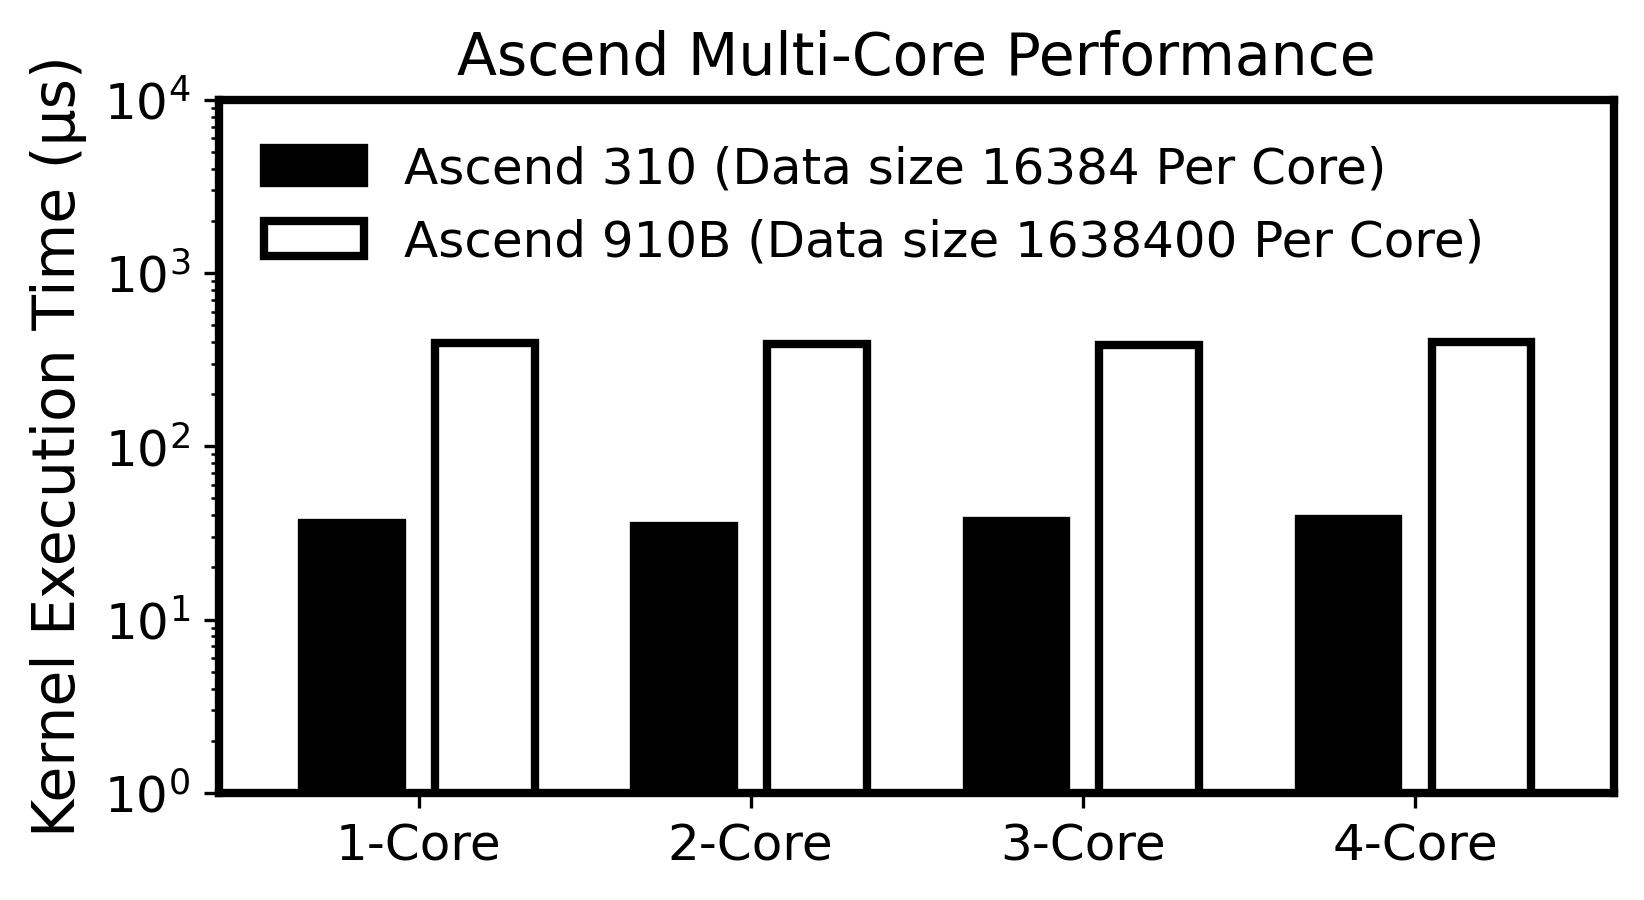
\includegraphics[scale=0.58]{figures/multi.png}}
    \caption{The multi-core execution of Cube-fx}
    \label{fig:multi}
    \end{figure}

As shown in Fig. \ref{fig:multi}, the performance of Cube-fx in multi-core environments shows no clear performance loss compared to the single-core case, which suggests that Cube-fx runs efficiently when multiple cores are used. This result can be attributed to Cube-fx being a data parallelism-based algorithm, allowing it to distribute workloads effectively among different cores and fully utilize the processors' resources. This ensures scalability and maintains high performance across multiple cores, taking full advantage of the parallel processing capabilities and maximizing overall system performance.

\subsection{Unfilled Matrix MAC Evaluation}

\begin{figure}[tbp]
    \centering{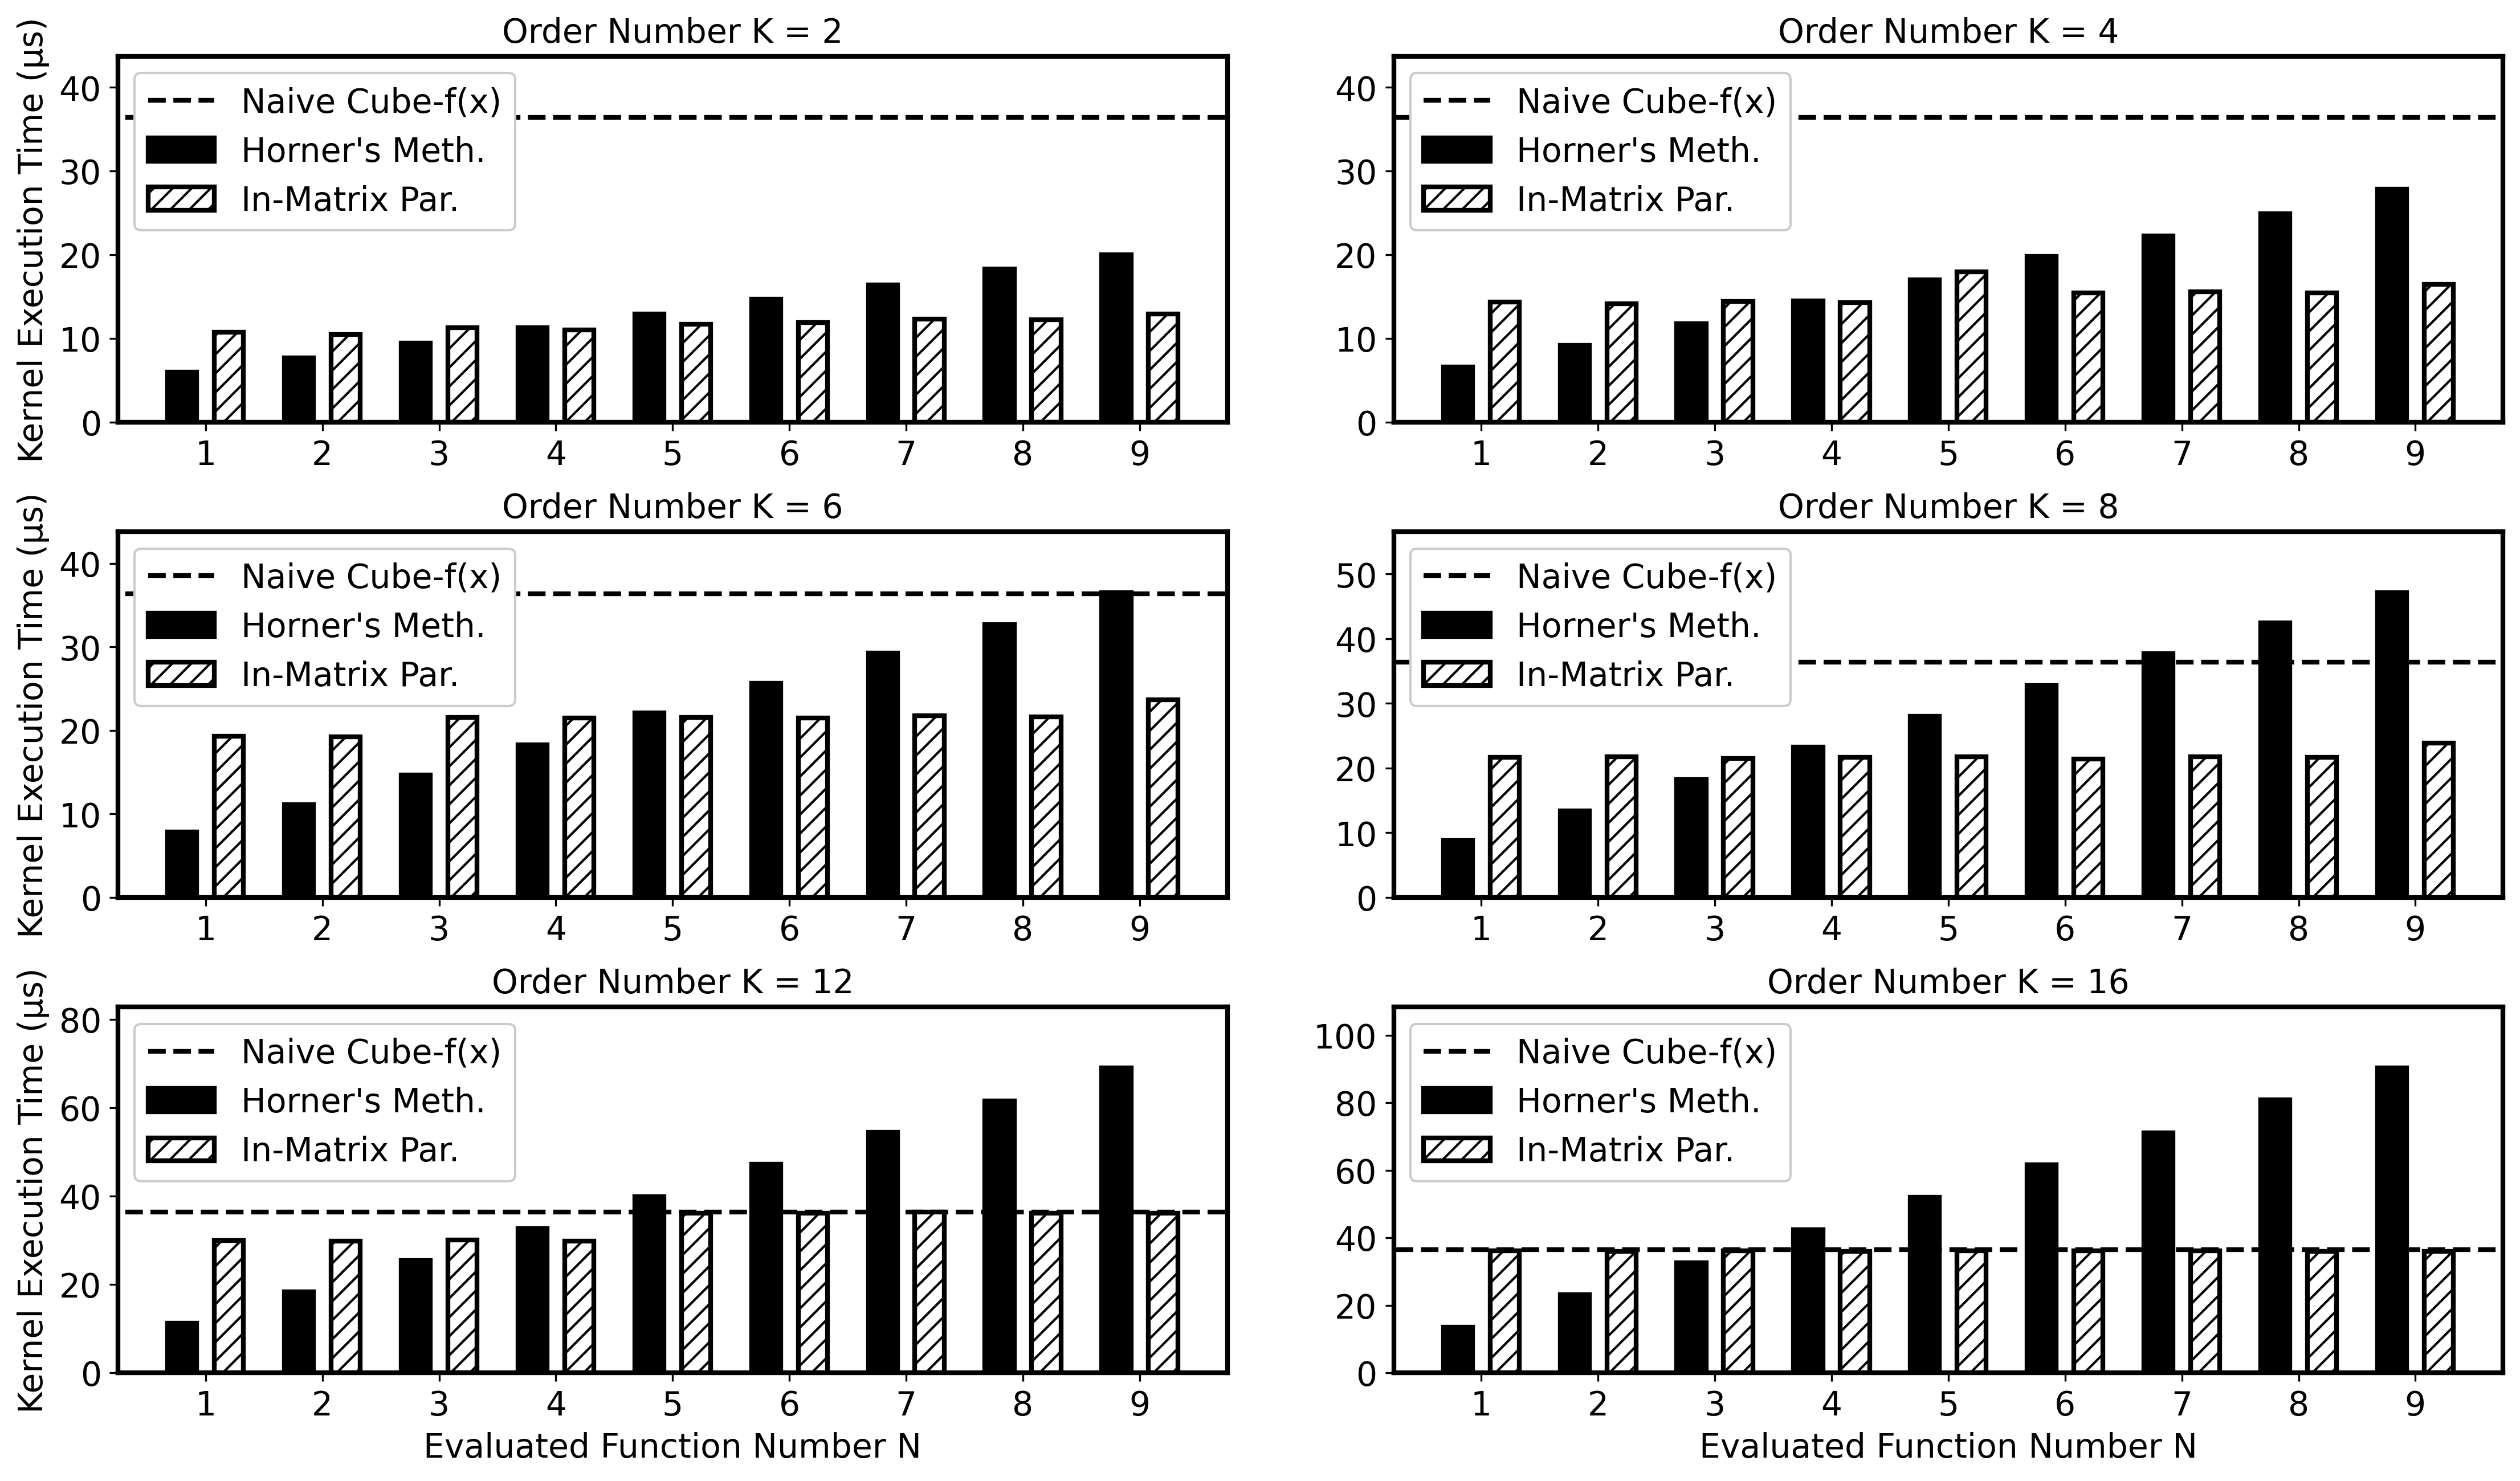
\includegraphics[scale=0.36]{figures/results.png}}
    \caption{The accelerations of the enhanced Cube-fx}
    \label{fig:results}
    \end{figure}

This subsection evaluates the performance of the enhanced Cube-fx on both Ascend 310 processors and Ascend 910B processors. For cases where $k = \{2, 6, 12\}$, the results are evaluated on Ascend 310 processors, while for cases where $k = \{4, 8, 16\}$, the results are evaluated on Ascend 910B processors. To indicate the performance improvement of the enhanced Cube-fx, we compare its execution time with those of Horner's Method, naive Cube-fx, and the enhanced Cube-fx with a fixed number of merged matrices $t = 4$. The data size used in this subsection is 16384 and 1638400, respectively, on Ascend 310 and Ascend 910B. 

Fig. \ref{fig:results} illustrates our collected evaluation results. Since the execution time of naive Cube-fx for all cases is the same, we plot it as a dashed line in all charts, which reports significant performance gaps between the other two implementations in most cases. Generally, the enhanced Cube-fx reports an average speedup of $1.83\times$ compared to naive Cube-fx on Ascend 310 processors and $1.63\times$ on Ascend 910B processors. While the best case reports a $3.39\times$ speedup on Ascend 310 processors and $2.68\%$ speedup on Ascend 910B processors, the worst reports an equivalent execution time compared to naive Cube-fx. Compared with the results of the enhanced Cube-fx when $t = 4$, the enhanced Cube-fx with the optimized $t$ reports an average speedup of $1.12\times$ and $1.28\times$. These results mean that applying the enhanced mapping to Cube-fx for all cases is riskless, and our optimized problem helps find the optimized execution of Cube-fx. Compared with Horner's Method on Ascend 310 processors, the enhanced mapping empowers Cube-fx again and offers the capability to beat Horner's Method. The enhanced Cube-fx reports lower execution time when the number of evaluated functions is larger than about 4, similar results to the saturated Matrix MAC results in Sec. \ref{Sec: 4.2}. However, on Ascend 910B processors, the enhanced Cube-fx cannot work as powerfully as on Ascend 310 processors. The reason is that Horner's Method works so well on Ascend 910B processors, as discussed in Sec. \ref{Sec: 4.2}, that Cube-fx can only outperforms when $k$ is large enough.

\subsection{Case Study: Audio Signal Feature Extraction}

In this subsection, we demonstrate how Cube-fx enhances the efficiency of feature extraction for real applications in audio signal processing \cite{deller1993discrete}. One-dimensional audio signals can be transformed using the Fourier transform to represent them as trigonometric functions, enabling Taylor expansion to evaluate the impact of small perturbations. For simplicity, our experiments directly use basic cosine signals as inputs. Table \ref{tab:app} presents several sample features used in the experiment. For features requiring multiple input values, such as Short-Time Autocorrelation, we employ a sliding window approach to generate input vectors from the original data for each window. All input data sizes are set to 16M for evaluation consistency.

\begin{table}[tbp]
  \caption{Sample features of audio signal}
  \label{tab:app}
  \begin{center}
  
  \scalebox{0.85}{
      \begin{tabular}{c|c}
      \toprule[1pt]
          \makecell[c]{\textbf{Feature}} &
          \makecell[c]{\textbf{Taylor Expansion of $x(t) = \cos(t)$}} \\
      \midrule[0.5pt]
  
      \makecell[c]{Instantaneous \\ Amplitude} &
      \makecell[c]{$
      A(t + \Delta t) = |\cos(t)| - \sin(t) \Delta t - \cos(t) \Delta t^2 / 2$ \\
      $+ \sin(t) \Delta t^3 / 6 + \cos(t) \Delta t^4 / 24 +  \dots$}
      \\
      \midrule[0.5pt]

      \makecell[c]{Log- \\ Amplitude} &
      \makecell[c]{$L(t + \Delta t) = \log(|\cos(t)|) - \tan(t) \Delta t - \Delta t^2 / (2\cos^2(t))$ \\
      $+ \tan(t) \Delta t^3 / (3\cos^2(t)) - \Delta t^4 / (4\cos^4(t)) \dots$}
      \\
      \midrule[0.5pt]

      \makecell[c]{Instantaneous \\ Power} &
      \makecell[c]{$P(t + \Delta t) = \cos^2(t) - 2\cos(t)\sin(t) \Delta t - \sin^2(t) \Delta t^2$ \\
      $+ 2\cos(t)\sin(t) \Delta t^3 / 3 + \sin^4(t) \Delta t^4 / 24 + \dots$} 
      \\
      \midrule[0.5pt]

      \makecell[c]{Instantaneous \\ Gradient} &
      \makecell[c]{$G(t + \Delta t) = -\sin(t) - \cos(t) \Delta t + \sin(t) \Delta t^2 / 2$ \\ 
      $+ \cos(t) \Delta t^3 / 6 - \sin(t) \Delta t^4 / 24 + \dots$}
      \\
      \midrule[0.5pt]

      \makecell[c]{Short-Time \\ Autocorrelation} &
      \makecell[c]{$R(\tau+\Delta t) = \sum_{t=0}^{T-1} \cos(t) \cdot$ \\ 
      $\left( \cos(t+\tau) - \sin(t+\tau) \Delta t - \cos(t+\tau) / 2 \Delta t^2 + \cdots \right)$}
      \\

      \bottomrule[1pt]
      \end{tabular}
  }
  
  \end{center}
  \end{table}

\begin{figure}[tbp]
  \centering{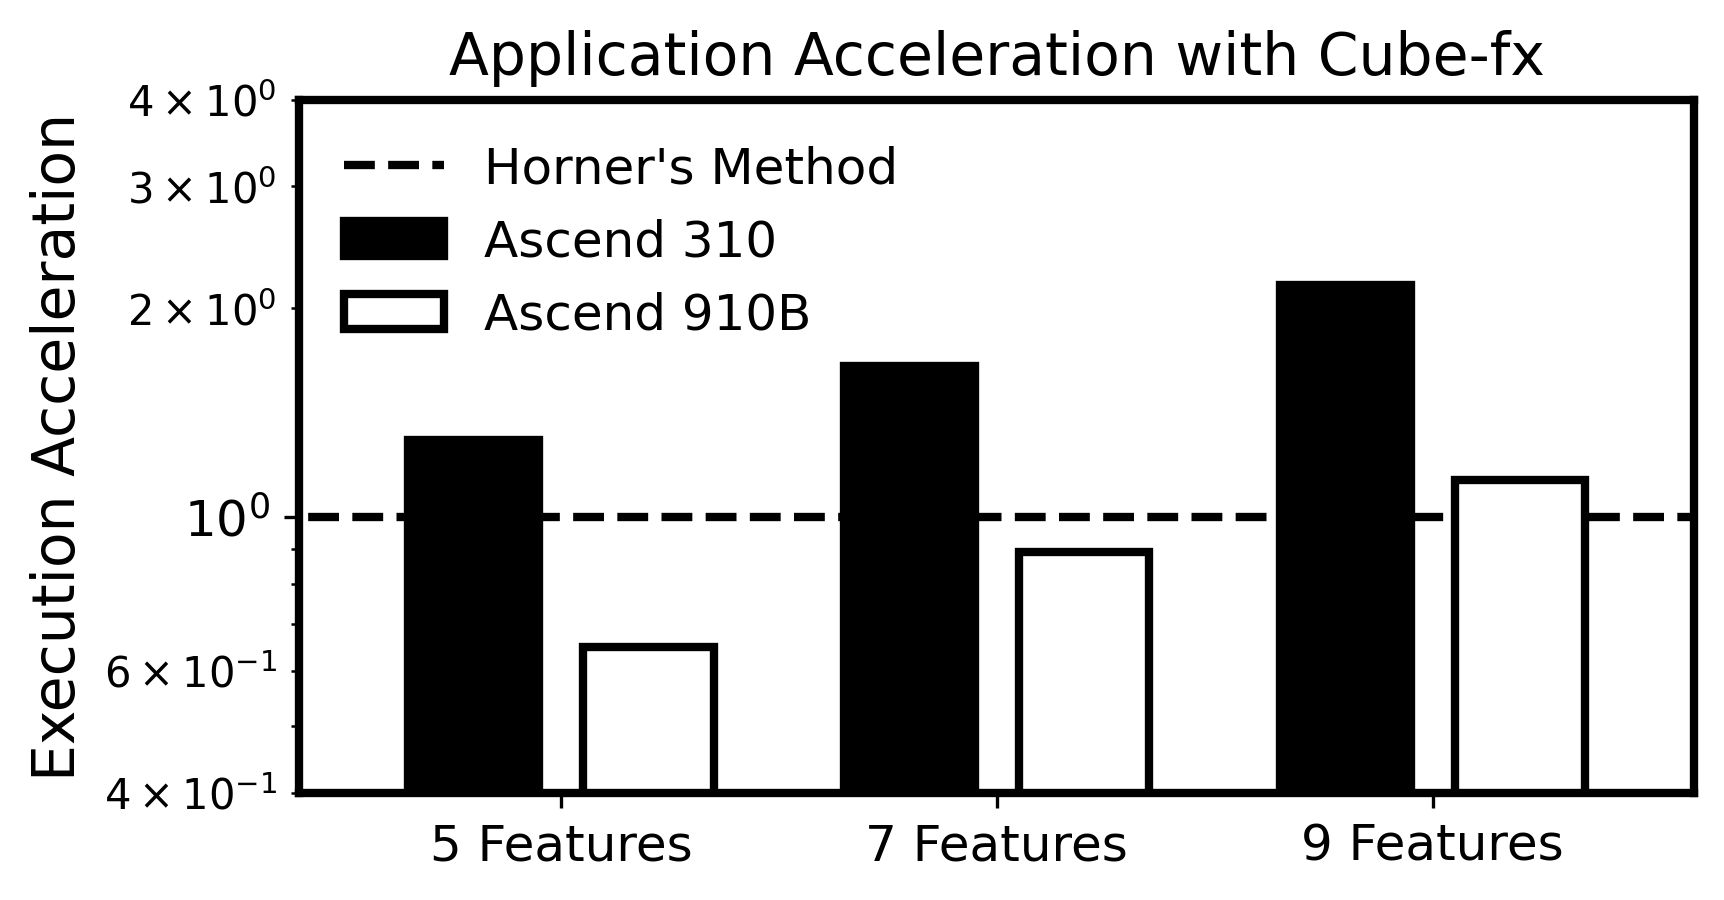
\includegraphics[scale=0.58]{figures/app_acc.png}}
  \caption{Feature extraction with Cube-fx acceleration in audio signal processing}
  \label{fig:app_acc_1}
  \end{figure}

Fig. \ref{fig:app_acc_1} presents the evaluation results for feature extraction in audio signal processing. Beacuse of the input vector generation required in this application, Cube-fx demonstrates slightly lower acceleration compared to previous experiments. Across the three experiments, the average speedup over Horner's Method is $1.70\times$ on the Ascend 310 processor and $0.89\times$ on the Ascend 910B processor. Specifically, while the previous benchmarking results indicated nearly identical performance for extracting 7 features in both implementations, the real application results reveal a noticeable performance drop caused by the input vector generation. These findings reaffirm our previous analysis in Sec \ref{sec:dis_1}: Cube-fx, with its reliance on extensive communication, performs efficiently on the Ascend 310 processor but faces challenges on the Ascend 910B processor.

\section{Conclusion \label{sec:8}}

This chapter introduced Cube-fx, a novel algorithm to map Taylor expansion for function evaluation onto the powerful Matrix MACs of the AI processors, especially the Huawei Ascend processors we focus on in this paper. Based on the fact that the AI processors usually equip poor vector units and a piece of data often needs to be computed by multiple functions in real-world applications, Cube-fx converts the building and computation of Taylor polynomials to specific matrix multiplications supported by the Matrix MACs. Since the Matrix MACs must complete a fixed shape of matrix multiplication each time, Cube-fx wastes a part of the computation power when the order number of Taylor polynomial is low. Therefore, we propose another further mapping technology to fuse the matrix multiplications of Cube-fx, which again empowers Cube-fx and exploits the computation power as much as possible. Although the application and performance of Cube-fx are still imperfect, our attempt to extend the programmability of the AI processors would inspire more researchers to work on this novel hardware with more valuable results.